%include part: see main.beamer.tex and main.article.tex
\usepackage{etex} %эта магическая херь избавляет от переполнения регистров TeX а!!!

\mode<article>{\usepackage{fullpage}}
\mode<presentation>{
    \usetheme{Madrid}
    \useoutertheme{shadow}
} 

\usepackage[utf8]{inputenc}
\usepackage[russian]{babel}
\usepackage{indentfirst}
\usepackage{graphicx}

\usepackage{amsmath}
\usepackage{amsfonts}
\usepackage{amsthm}
%\usepackage{algorithm}
%\usepackage{algorithmic}

%\usepackage[all]{xy}

\date{Лекция по дисциплине <<методы и средства защиты компьютерной информации>> (\today)}
\author[М.~М.~Шихов]{Михаил Шихов \\ \texttt{\underline{m.m.shihov@gmail.com}}}

%%для рисования графов пакетом xy-pic
%\entrymodifiers={++[o][F-]}

%%для псевдокода алгоритмов (algorithm,algorithmic)
%\renewcommand{\algorithmicrequire}{\textbf{Вход:}}
%\renewcommand{\algorithmicensure}{\textbf{Выход:}}
%\renewcommand{\algorithmiccomment}[1]{// #1}
%\floatname{algorithm}{Псевдокод}

%\setbeamercolor{alerted text}{fg=-green} %gyan, blue, green, -green

\title[Объект защиты --- информация]{Объект защиты --- информация}


\begin{document}


%титул и содержание статьи
\mode<article>{\maketitle\tableofcontents}

%титул и содержание презентации
\frame<presentation>{\titlepage}
\begin{frame}<presentation>[allowframebreaks]
    \frametitle{Содержание}
    \tableofcontents
\end{frame}


\section{Информация}


\subsection{Определения}


Исторически слово информация (informatio) пришло в наш язык из латинского и дословно означает <<осведомлять>>. Но время не стоит на месте, и теперь практически в каждой прикладной области используется свое <<удобное>> определение этому термину.
Например, характерными определениями информации в \emph{экономике} являются следующие:
\begin{itemize}
    \item информация это сведения, данные, значения экономических показателей, являющиеся объектами хранения, обработки и передачи и используемые в процессе анализа и выработки экономических решений в управлении; 
    \item информация это один из видов ресурсов, используемых в экономических процессах, получение которого требует затрат времени и других видов ресурсов, в связи с чем эти затраты следует включать в издержки производства и обращения. 
\end{itemize}

В толковом словаре по вычислительной технике В. Иллингуорта, Э.Л. Глейзера и И.К. Пайла приводится определение, удобное для специалистов в области информатики и вычислительной техники, которое мы примем за основу: 

\begin{frame}
    \frametitle{Определения}
    
    Данное определение информации примем за основу:
    \begin{definition}
        \alert{Информация} --- это совокупность (цепочка) \alert{символов}. В свою очередь, \alert{символы} определяются как образы, несущие смысловую нагрузку
    \end{definition}

    Данное определение установлено законом\footnote{№149-ФЗ от 27 июля 2006 г <<Об информации, информационных технологиях и о защите информации>>}:
    \begin{definition}
        \alert{Информация} --- это сведения (сообщения, данные) независимо от формы их представления
    \end{definition}
\end{frame}

Примеры определений можно приводить очень долго, но, конечно, «универсальное» для общества определение этому термину следует искать в области закона. Интересен тот факт, что хотя в конституции (ст. 29,п.4) и гражданском кодексе (ст. 128) и указано, что информация является одним из видов гражданских прав, но определения, что такое информации там нет. Четкое определение находим в достаточно специфичном Федеральном законе РФ №149 от 27 июля 2006 г «Об информации, информационных технологиях и о защите информации»: «информация это сведения (сообщения, данные) независимо от формы их представления». 

Информации сложно дать единое, максимально общее качественное определение в силу фундаментальности понятия. «Отец кибернетики» Норберт Винер дал, например, такое определение: «Информация есть информация, а не материя или энергия». Но отделяя понятие информации от материи и энергии, конечно нельзя забывать о тонкой взаимосвязи этих понятий. Создание, передача, сохранение, копирование, обработка, защита, уничтожение и прочие действия в отношении информации требуют затрат и материи и энергии. 

Одна и та же информация может быть представлена в различной материально-энергетической форме, например, в световых, звуковых и радиоволнах, в уровнях электрического тока или напряжения, в напряженностях магнитного поля, в знаках и изображениях на подходящей поверхности и т.д. С помощью весьма ограниченного набора органов чувств (зрение, слух, обоняние, вкус, осязание, чувство равновесия) человек воспринимает бесконечно малую толику из всех возможных форм представления информации. И после совершенно незаметного чуда, превращающего воспринятое в информацию, законопослушному её обладателю становится ясно, что с точки зрения закона уже совершенно не важно, как эта информация была представлена до её получения.


\subsection{Точки зрения на информацию}


Если принять определение, что информация это набор символов, которым соответствуют образы, несущие некоторую смысловую нагрузку, то такой набор удобно рассматривать с трех точек зрения.

\begin{frame}
\frametitle{Точки зрения на информацию}
\begin{itemize}
    \item Поведенческая.
    \mode<article> {
        Важным с этой точки зрения является то, что любые действия (например, создание, получение, передача, обработка и т.д.) над информацией имеют определенные причины, а результат этих действий повлечет в свою очередь определенные следствия. Например, можно оценивать поведение мыслящего существа или отклики автоматической системы вследствие получения ими определенной информации.
    }
    
    \item Математико-лингвистическая.
    \mode<article> {
        В этом случае важна структура набора символов и его смысловое содержание. Обладая информацией о структуре и соотнося её с конкретным набором символов, мы можем выделять из этого набора подгруппы символов, несущих совокупную смысловую нагрузку, и таким образом переходить к смысловому содержанию всего набора в целом. Например, с этой точки зрения смотрят на информацию, разбираясь в исходном тексте программы, или анализируя формат файла, содержащего музыкальные или графические данные и т.д.
    }
    
    \item Физико-техническая.
    \mode<article> {
        Пристальный взгляд направлен, очевидно, на физические и технические аспекты представления информации. То есть важно, в какой материально-энергетической форме информация представлена, технические способы воздействия на представление информации, количественные оценки информации с точки зрения технических затрат и т.д. Взгляните с этой точки зрения, например, на процесс записи концерта: как преобразовать информацию, представленную в колебаниях воздуха, в эквивалент на flash-накопителе вашего mp3 плеера?
    }
\end{itemize}
\end{frame}


\subsection{Свойства информации}


\begin{frame}
    \frametitle{Свойства информации}
    \begin{figure}
        \begin{center}
            \mode<presentation>{ 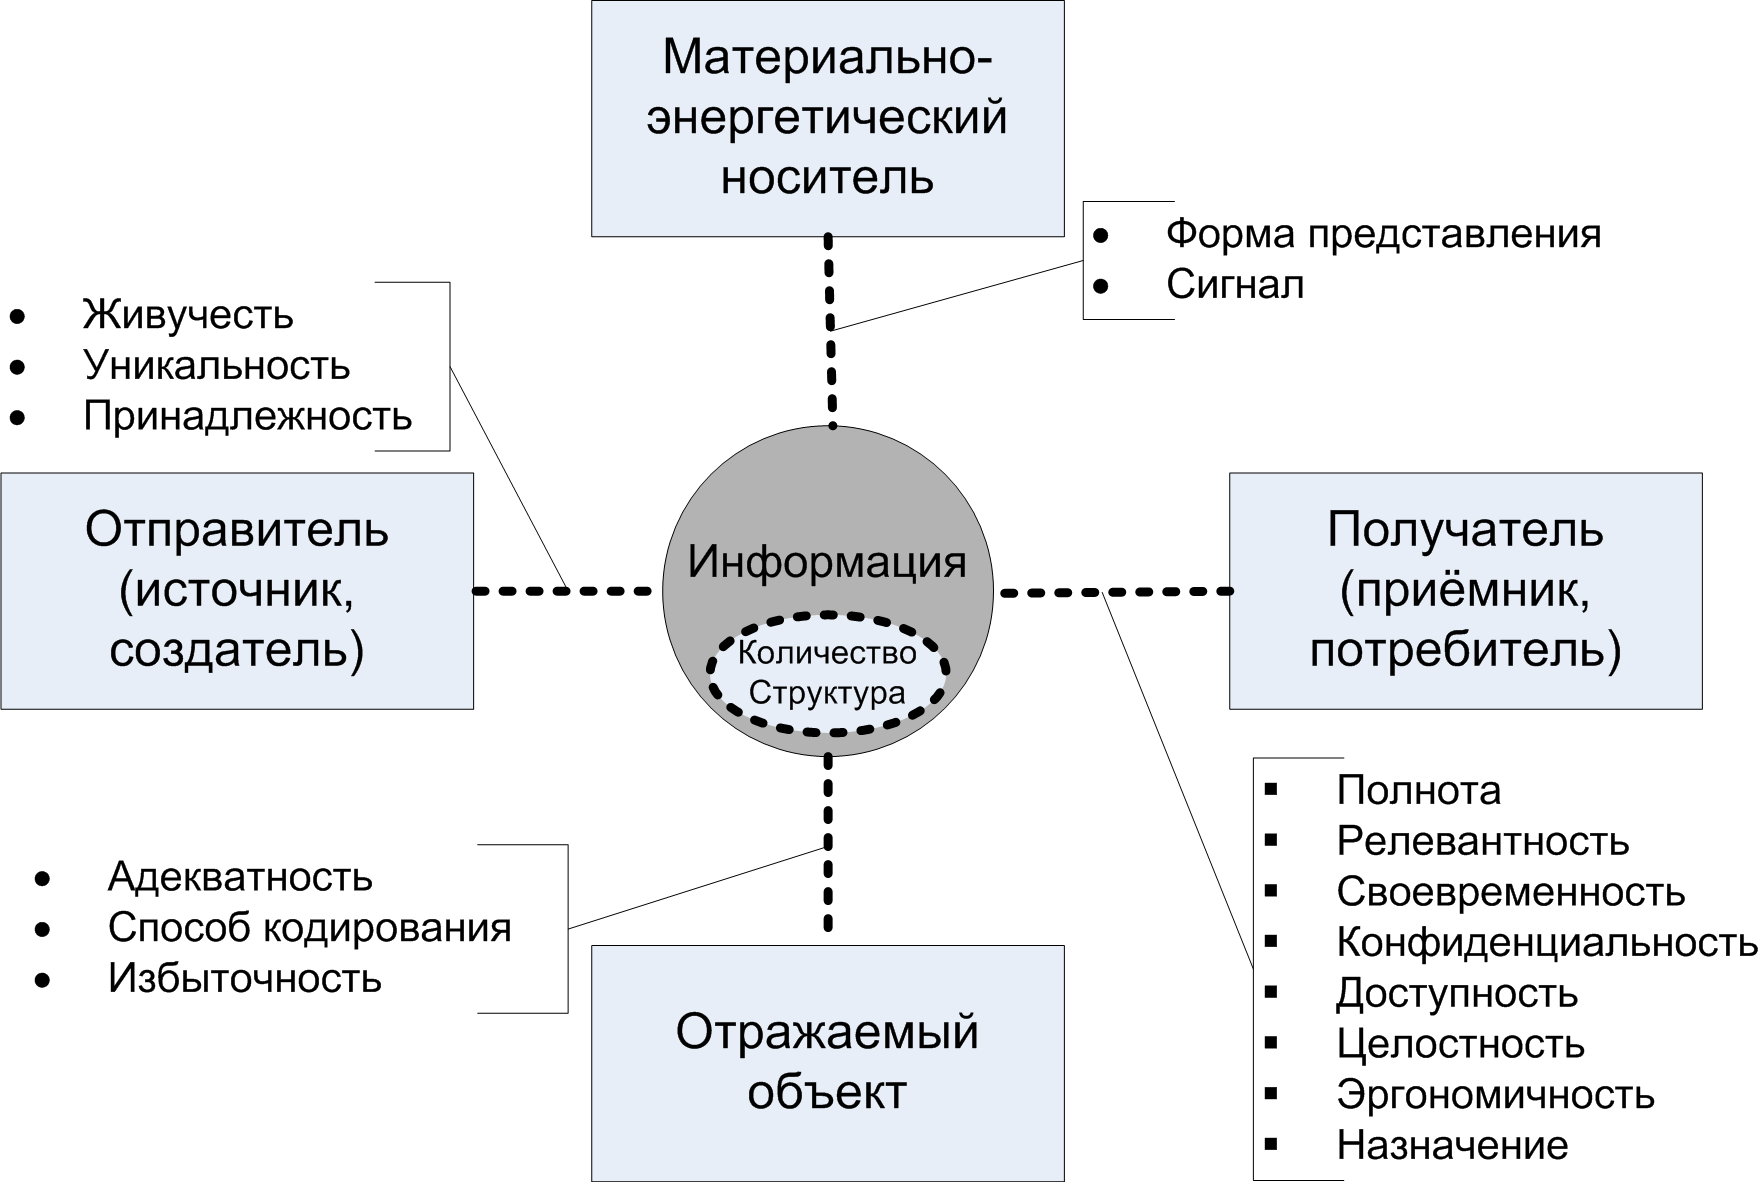
\includegraphics[height=.75\textheight]{pict/iproperties} }
            \mode<article>{ 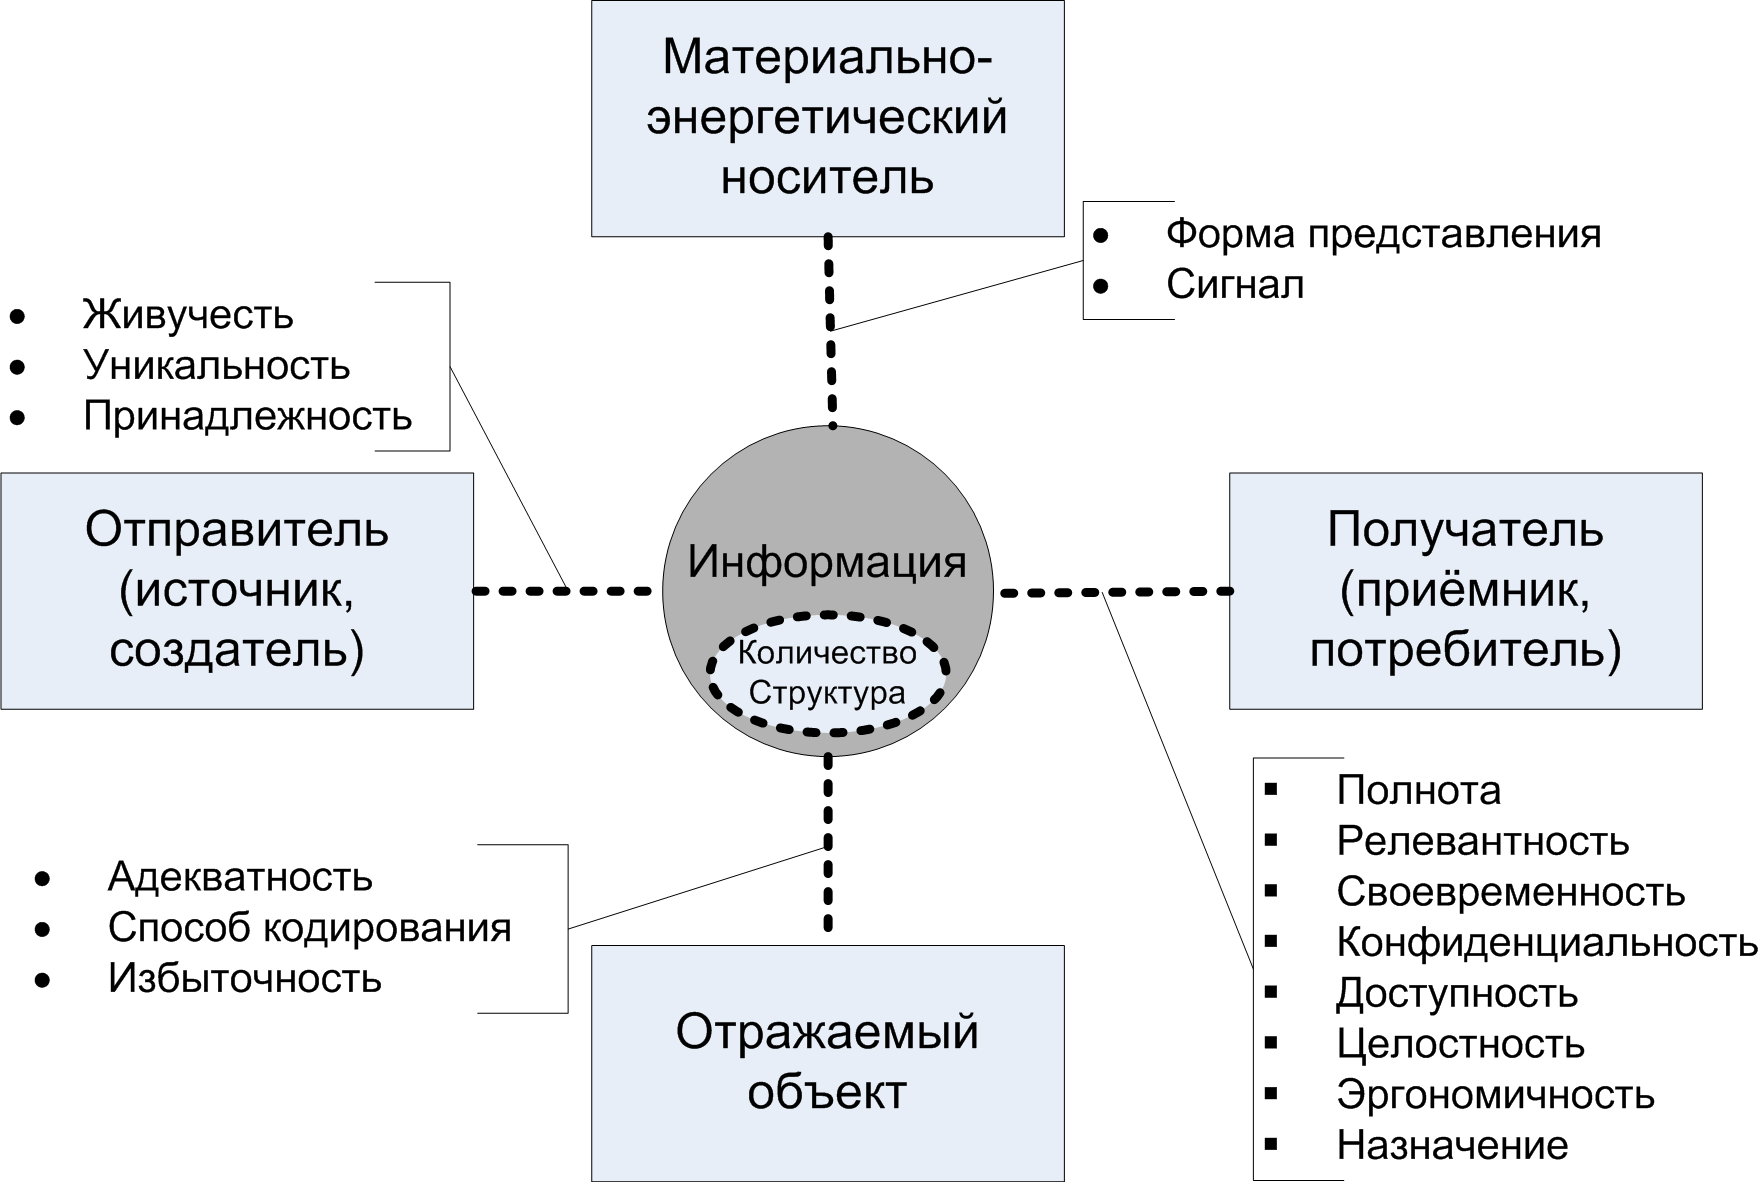
\includegraphics[width=.8\textwidth]{pict/iproperties} } 
        \end{center}
        \caption{Свойства информации}\label{pict:iproperties}
    \end{figure} 
    \mode<article>{ См. рисунок \ref{pict:iproperties} }
\end{frame}


Обычно, рассматривая нечто как объект, полезно выделить внутренние и внешние свойства этого объекта. Внутренние свойства органически присущи объекту и характеризуют его вне зависимости от его взаимодействия с другими объектами. Внешние же свойства характеризуют объект при его взаимодействии с другими объектами и не имеют смысла в отсутствие такого взаимодействия.

Рассматривая информацию как объект (см. рис. \ref{pict:iproperties}), мы выделим два важнейших \emph{внутренних} её свойства, которым в дальнейшем уделим самое пристальное внимание, – это \emph{количество} (или объем) и \emph{структура} (или внутренняя организация) информации. 
О внешних свойствах придется говорить в контексте её отношений с другими объектами, из которых особо мы выделим следующие:
\begin{itemize}
    \item \emph{отправитель}, он же автор, создатель, источник;
    \item \emph{получатель}, он же приемник или потребитель;
    \item \emph{материально-энергетический носитель} информации, без которого, как уже ясно, отправитель не отправит, а получатель не получит информацию;
    \item отражаемый объект, некоторый объект, в отношении которого между отправителем и получателем идет информационный обмен.
\end{itemize}


Раскроем вкратце суть некоторых внешних свойств информации. Часть из этих свойств можно определить количественно, то есть измерить, выразить числом, а часть можно определить только на качественном уровне.

Самая многочисленная группа внешних свойств проявляется в отношении \emph{получателя}. \emph{Полнота} --- свойство информации исчерпывающе характеризовать получателю отражаемый объект. \emph{Релевантность} --- свойство соответствовать нуждам (запросам) потребителя. \emph{Своевременность} --- это релевантность в нужный момент времени. \emph{Конфиденциальность} --- недоступность третьим лицам\footnote{Напомним русский язык. Первое лицо: я, мы, Второе лицо: ты, вы. И третье: он, она, оно, они.} (не исключает доступность). \emph{Доступность} --- свойство информации быть доступной законному потребителю (т.е. первым и вторым лицам, что, конечно не исключает конфиденциальности). \emph{Целостность} --- свойство неизменности относительно некоторого фиксированного значения (например, это свойство дает получателю уверенность в том, что он получил информацию в том виде, в котором она была отправлена). \emph{Эргономичность} --- удобство избранных свойств (как внешних, так и внутренних) информации для потребителя. \emph{Назначение} --- свойство, отражающее полезность информации для потребителя-специалиста в определенной области (экономическая, техническая, биологическая, статистическая, генетическая и пр. информация).

В отношении \emph{отправителя} можно выделить следующие свойства информации. \emph{Живучесть} --- свойство информации, находясь в источнике, сохранять свои внутренние свойства с течением времени. \emph{Уникальность} --- уверенность в существовании единственного источника информации, никогда не осуществлявшего её передачу. \emph{Принадлежность} --- свойство информации, позволяющее определить её источник или факт её получения приемником (в этом случае это внешнее свойство проявляется в отношении отправителя и получателя сразу).

Одним из важнейших свойств информации в отношении \emph{отражаемого объекта} является \emph{адекватность}. Понятие отражаемый объект следует понимать максимально широко: это может быть все, что угодно: другая информация, процесс, явление, ситуация, предмет и т.д.  \emph{Адекватность} --- это свойство информации однозначно соответствовать отражаемому объекту. \emph{Способ кодирования} --- способ, определяющий возможность перехода от отражаемого объекта к информации (обратный переход от информации к объекту называется \emph{декодированием}). \emph{Избыточностью} называется превышение количества информации, над необходимым минимумом для \emph{адекватного} соответствия \emph{отражаемому объекту}.

В отношении \emph{материально-энергетического носителя} очевидное свойство --- \emph{форма представления} информации (собственно сам носитель этой формой и является). \emph{Сигнал} --- это изменение (во времени или пространстве) физической величины, несущее информацию, т.е.  способ позволяющий фиксировать \emph{символ} в материально-энергетическом носителе (напомним, что результатом кодирования является набор символов --- это есть информация). 


\begin{frame}
\frametitle{Свойства информации, подлежащие защите}
\begin{itemize}
    \item \alert{Конфиденциальность}.
    \item \alert{Целостность}.
    \item \alert{Доступность}.
    \item \alert{Принадлежность}.
\end{itemize} 
\end{frame}



\section{Количественные оценки}

Как мы уже знаем, единой точки зрения на информацию нет, нет и единого подхода к оценке свойств информации. Выделяют следующие подходы: синтаксический, семантический, прагматический.

\begin{frame}
\frametitle{Подходы к количественной оценке информации}
\begin{itemize}
    \item Синтаксический. \mode<article>{Синтаксический подход дает оценку информации, учитывая только \emph{структурные} особенности отражаемого объекта.}
    
    \item Семантический. \mode<article>{Семантический дает оценку, учитывая \emph{смысловую нагрузку}, которую несет отражаемый объект для потребителя его информационного отражения.}
    
    \item Прагматический. \mode<article>{Прагматический подход дает оценку, учитывая полезность отражаемого объекта для потребителя в процессе достижения некоторой \emph{цели}.}
\end{itemize} 
\end{frame}


Многие свойства информации (как внутренние, так и внешние) можно оценить количественно. На примере такого внутреннего свойства информации как её количество, покажем, что задача количественной оценки отнюдь не проста.

Если мы примем определение, что информация --- это совокупность символов, то её количество оценивается тривиально. Количество информации = количество символов в совокупности. Единица измерения --- символ. 

Казалось бы: вот и все! Чего еще думать? Думать действительно нечего, если вы потребитель информации. Но вот если вы создатель (автор), то подумать придется: в отношении создателя внутренне свойство <<количество>> не проявляется столь явно в силу того, что самой информации попросту пока нет! Есть только отражаемый объект, и требуется создать его отражение --- информацию. Каково будет её количество --- открытый вопрос.

Забегая вперед, отметим, что мы привыкли измерять информацию в битах. Битом называют любой символ из множества, состоящего двух различных символов (обычно 0 и 1). Смысловая нагрузка бита: ответ либо да (символ 1), либо нет (символ 0) на вопрос об отражаемом объекте. На основе бита выстраиваются более крупные единицы информации: байты, килобайты, кибибайты, мегабайты, мебибайты, и тд\ldots Подробнее об этом далее.

Допустим, вам принесли цифровую стереофотографию, то есть информацию, объемом 127 мегабайт. У вас не возникает затруднений оценить, получится ли её сохранить на своем компьютере. Но оглянитесь вокруг. Сможете ли вы оценить объем информации, хотя бы с точностью до десятка мегабайт, которая необходима для того, чтобы отразить в ней объемную фотографию окружающей вас обстановки?
Итак, трудности представляет оценка того, какое количество информации несет в себе тот или иной отражаемый объект? Точнее: какое количество этой информации необходимо и достаточно, чтобы адекватно отразить объект для потребителя? Поэтому далее мы будем говорить о количестве информации именно в контексте создания информации, то есть перехода от отражаемого объекта к информации. Этот переход называется \emph{кодированием}.

Оценку количества информации, необходимого для отражения, наиболее четко дает синтаксический подход. В действительности же все указанные подходы количественно оценивают внешнее свойство адекватности информации. Синтаксический подход оценивает адекватность отражения структурных свойств объекта. Семантический подход оценивает адекватность отражения объекта в контексте смысловых единиц, знаний, которыми обладает потребитель. Прагматический же подход дает оценку адекватности информации в процессе достижения потребителем определенной цели.


\subsection{Синтаксический подход}

Особое внимание мы уделим синтаксическому подходу. В подавляющем большинстве практических случаев кодирование осуществляется на его основе. В рамках этого подхода упрощенно рассмотрим оценки американских ученых Ральфа Хартли и Клода Шеннона.
Отражаемый объект рассматривается как источник, но не информации, а событий, снимающих неопределенность о его структуре. В качестве примера приведем задачу о картах.

\begin{frame}
\frametitle{Задача о картах}
\framesubtitle{Постановка задачи}
\begin{example}
    Имеется колода из восьми карт. По две карты (допустим, туз и двойка) каждой масти. Профессор вытягивает наугад карту и готов честно давать ответы да/нет на любые задаваемые вопросы. Нужно минимальным количеством вопросов угадать вытащенную карту.
\end{example} 
\end{frame}

Итак. Имеем отражаемый объект --- это колода карт, из которой вытащили одну карту. Неопределенность о структуре этой неполной колоды снимается, когда становится ясно, какая карта была вытащена. Источником событий  служит профессор, а его ответы да/нет являются событиями.

Можно решить задачу ГСН\footnote{ГСН метод --- метод Грубой Силы и Невежества} методом: задавать вопросы о конкретной карте. Тогда можно угадать карту и одним вопросом, но вероятность тому весьма мала. В худшем же случае потребуется семь вопросов. 

Более <<тонкое>> решение: каждым вопросом сокращать неопределенность вдвое. Например, ответ на первый вопрос о цвете масти разделит нам исходную колоду на две равные части по четыре карты.  Вопрос о конкретной масти оставит нам две карты. И вопрос о достоинстве карты будет последним. См. рисунок \ref{pict:cards}

\begin{frame}
\frametitle{Задача о картах}
\framesubtitle{Решение}
\begin{figure}
    \begin{center}
        \mode<presentation>{ 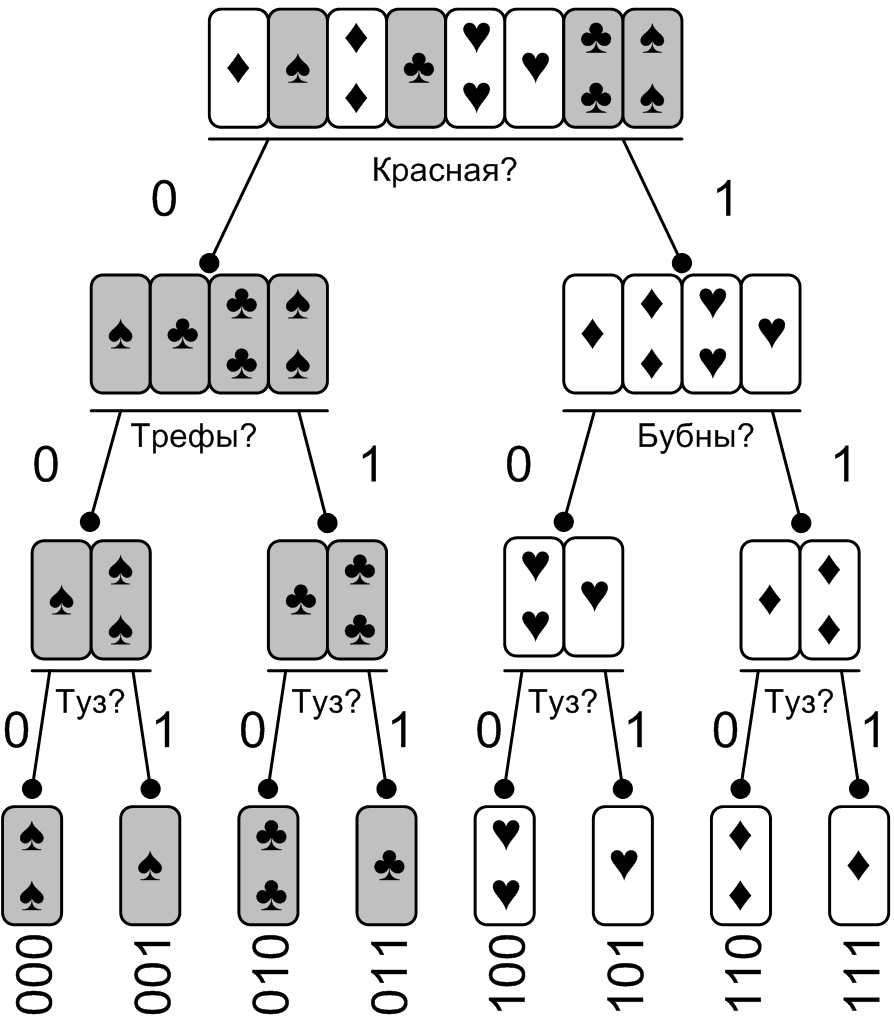
\includegraphics[height=.7\textheight]{pict/cards} }
        \mode<article>{ 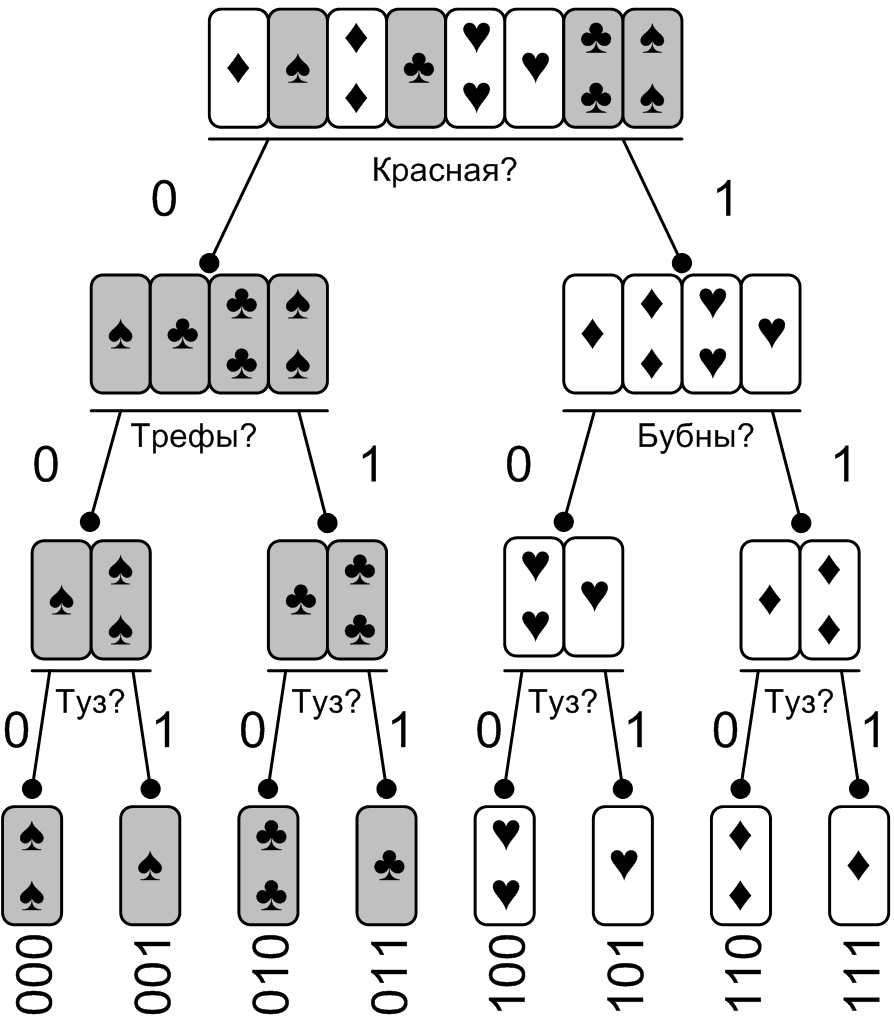
\includegraphics[width=.4\textwidth]{pict/cards} } 
    \end{center}
    \caption{Кодирование в задаче о картах}\label{pict:cards}
\end{figure} 
\mode<article>{ См. рисунок \ref{pict:cards} }
\end{frame}

А теперь выполним переход к информации. Каждому событию-ответу мы поставим в соответствие символ: событию да – символ 1, событию нет – символ 0. Двигаясь от вершины полученного дерева (Рис. \ref{pict:cards}) до конкретной карты, формируем соответствующую ей цепочку символов. Теперь цепочка из трех символов-бит полностью отражает структуру колоды карт. Итак, исходя только из структурных свойств колоды, мы выполнили оценку количества необходимой информации: три бита.

Теперь, чтобы не утруждать себя вопросами, можно попросить профессора так же честно сообщить информацию о вытащенной карте. И если он передал вам записанную на бумажке цепочку символов 011 (одно сообщение!), вы без труда догадаетесь, что в колоде не хватает туза треф.

Обобщая пример, вернемся к мере Ральфа Хартли. Пусть у нас имеется конечный набор символов. Количество символов в наборе --- $m$. Количество возможных комбинаций структуры (будем говорить просто: количество состояний) отражаемого объекта --- $N$. Итак, одним символом можно отразить $m$ состояний, двумя $m\cdot m=m^2$, тремя $m^3$, и т.д., цепочкой длины $H$ можно отразить $m^H$ состояний. Конечно, в практических целях нам нужно будет подобрать цепочку такой длины $H$, чтобы $m^H\geq N$. Мера же информации Ральфа Хартли, которая вовсе не обязана быть целым числом, предполагает $m^H=N$:


\begin{frame}
\frametitle{Мера Ральфа Хартли}
\begin{equation}
H=\log_{m}N,
\label{eq:hartley}
\end{equation}
где $m$ --- количество кодовых \alert{символов}; $N$ --- количество состояний \alert{отражаемого объекта}.

В ряде источников можно увидеть такой вариант:
\begin{equation}
H=\frac{\ln N}{\ln m},
\label{eq:hartleyln}
\end{equation}
где $H$ --- мера Хартли, $\ln X$ --- обозначение натурального (по основанию $e$) логарифма от $X$.

\begin{example}
В случае примера с картами: количество состояний $N=8$, количество символов $m=2$. Количество информации по Хартли: $H=\log_{2}8=3$ бита.
\end{example}
\end{frame}


Примерно через двадцать лет после работ Ральфа Хартли, его соотечественник Клод Шеннон ввел в 1948 г. более общую меру. При этом мера Хартли не утратила своей ценности и является важным частным случаем оценки по Шеннону. Приведем основные постулаты меры Шеннона.


\begin{frame}
    \frametitle{Мера Клода Шеннона}

    \begin{enumerate}
        \item Количество информации есть непрерывная функция от вероятности события.

        \item Количество информации $I_i$ одиночного $i$-го события $s_i$, $1\leq i\leq N$ происходящего с вероятностью $p_i$, имеет положительное значение. 
        \[I_i\geq 0; I_i=I(p_i), \sum_{i=1}^{N}p_i = 1\]

        \item Совместное количество информации $I_{ij}$ двух независимых событий $s_i, s_j$ с совместной вероятностью $p_{ij}=p_i\cdot p_j$, равно сумме их количеств информаций: 
        \(I_{ij}=I_i+I_j; I(p_i\cdot p_j)=I(p_i) + I(p_j).\)
    \end{enumerate}

    Всем этим свойствам удовлетворяет функция
    \begin{equation}
        I(p)=-\log_{m}(p),
        \label{eq:shannon}
    \end{equation}
    где $m>1$; $p$ --- вероятность события, несущего информацию $I(p)$.
\end{frame}


Итак, количество информации зависит от вероятности наступления события. Сравните свои эмоции от двух событий: <<Жучка укусила Иванова>> и <<Иванов укусил Жучку>>. Первое событие, хоть собака и друг человека, будничное, а вот второе вызывает улыбку --- сенсация! Вероятность первого события весьма велика, вероятность второго близка к нулю. Первое событие несет мало информации, а второе несет большое её количество, отсюда и эмоции.

В то же время, если мы услышим, что некий Шарик был искусан Петровым и Сидоровым\ldots Да, при вероятности в $0.001$ быть покусанным человеком Шарик мог быть уверенным, что его молнией убъет раньше, чем он доживет до дня, когда его покусают двое, потому как вероятность тому $0.000001$. Тем не менее мы получили всего лишь в два раза больше информации по сравнению с инцидентом с Жучкой, а не в $1000$. Потому никто, кроме Шарика не упадет в обморок от совместного оскорбления действием.

График зависимости информации от вероятности приведен на Рис.\ref{pict:ip}. При стремлении вероятности события $p$ к нулю, количество информации стремится к бесконечности. Событие с вероятностью 1 (происходящее всегда) не несет информации $I(1)=0$.

\begin{frame}
\frametitle{Зависимость количества информации от вероятности}
\begin{figure}
    \begin{center}
        \mode<presentation>{ 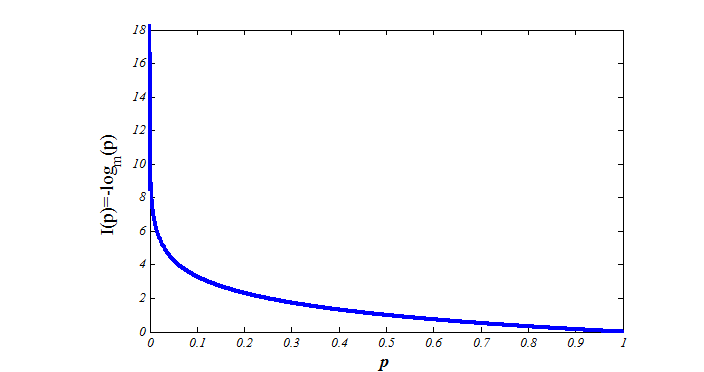
\includegraphics[height=.75\textheight]{pict/ip} }
        \mode<article>{ 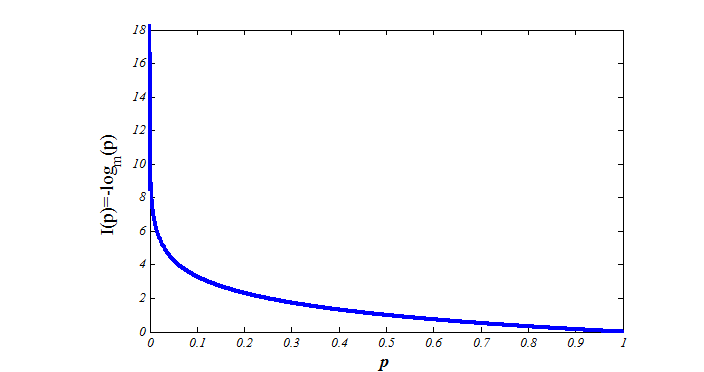
\includegraphics[width=.4\textwidth]{pict/ip} } 
    \end{center}
    \caption{Зависимость количества информации от вероятности}\label{pict:ip}
\end{figure} 
\mode<article>{ См. рисунок \ref{pict:ip} }
\end{frame}

В работе Шеннона вводится важная характеристика источника событий: энтропия. Энтропия --- мера неопределенности источника в целом. Энтропия играет важную роль в оптимальном кодировании, которое подробнее будет обсуждаться в дальнейшем. Проясним смысл понятия на примере источника, для которого известны вероятности поступления событий (источник без памяти в работе Шеннона). Допустим, что мы начали наблюдать за таким источником. Зададимся вопросом: <<сколько информации этот источник выдает в среднем?>>. Если мы наблюдали $M$ событий, то событие $s_i$ должно было произойти примерно  $p_i\cdot M$ раз. Если всего источник выдает $N$ событий (т.е. $i\in[1,N]$), то за весь период наблюдений он выдал примерно такое количество информации:
\[I\approx -\sum_{i=1}^{N}(p_i\cdot M) \cdot \log_{m}p_i.\]
В среднем же, каждым событием, источник выдавал количество информации равное $E=\frac{I}{M}$ см. формулу (\ref{eq:e}).

\begin{frame}
\frametitle{Энтропия}
\begin{equation}
    E=-\sum_{i=1}^{N}p_{i}\cdot \log_{m}p_i.
    \label{eq:e}
\end{equation}
\begin{figure}
    \begin{center}
        \mode<presentation>{ 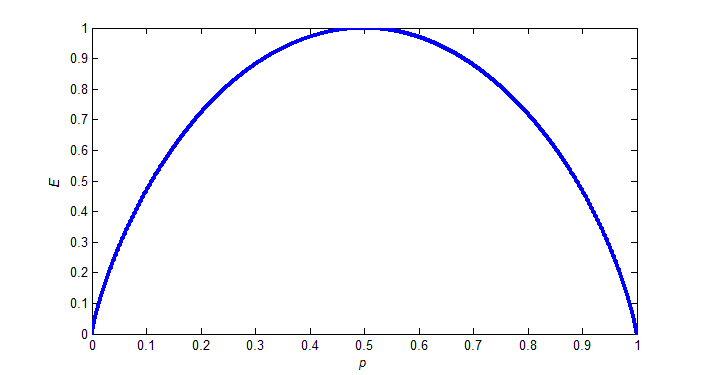
\includegraphics[height=.5\textheight]{pict/ecoin} }
        \mode<article>{ 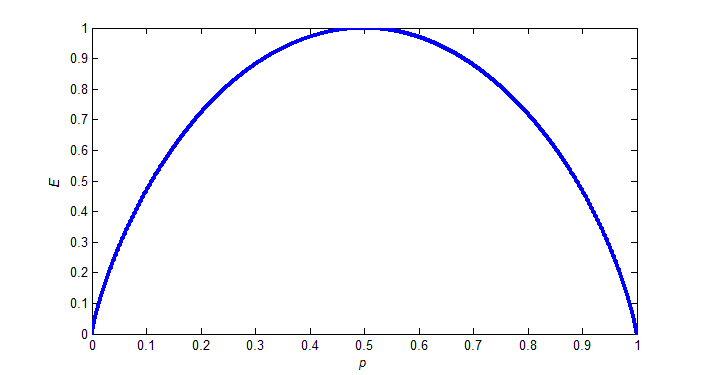
\includegraphics[width=.4\textwidth]{pict/ecoin} } 
    \end{center}
    \caption{Энтропия для источника с двумя состояниями}\label{pict:ecoin}
\end{figure} 
\mode<article>{ См. рисунок \ref{pict:ecoin} }
\end{frame}

Это значение и есть энтропия источника. Измеряется она в тех же единицах, что и информация. Максимум энтропии, а значит и неопределенности источника, достигается в том случае, когда все события равновероятны. Например, у нас есть источник-монетка: <<орёл>> выпадает с вероятностью $p$, а «решка», соответственно, с вероятностью $1-p$. График энтропии для монетки, как зависимость энтропии от вероятности выпадения «орла» представлен на Рис. \ref{pict:ecoin}. Видно, что максимума энтропия (неопределенность) достигает, когда вероятности выпадения «орла» и «решки» равны 0.5. Это значит что, если вы искренне хотите доверить некоторое решение судьбе, то возьмете монетку с максимальной неопределенностью, а если хотите заработать состояние, то возьмете монетку с нулевой неопределенностью, которая, например, всегда выпадает <<орлом>>, и разорите ближайшее казино.

Почему понятие энтропии столь важно? Создавая источник информации, эквивалентный источнику событий (то есть, например, в том же порядке выдающий информационные цепочки символов – отражения событий), важно помнить, что неопределенность (энтропия) источника информации  не может быть меньше неопределенности источника событий. Значение энтропии задает нижний предел неопределенности создаваемого источника информации. На практике неопределенность источника информации всегда больше неопределенности отражаемого источника сообщений и может лишь в той или иной мере к ней приближаться.

Итак, синтаксический подход дает нам возможность определять количество информации, необходимое для создания информационного дубликата отражаемого объекта. В каких же единицах это количество измеряется? Это зависит от того, сколько различных символов используется для составления информационной цепочки. Значение основания логарифма $m$ в формуле (\ref(eq:hartley)) (Хартли) и в формуле (\ref{eq:shannon}) (Шеннон) определяет единицу измерения. И лишь немногим значениям $m$ из бесконечного множества целых чисел история дала имя для соответствующей единицы измерения. О счастливчиках и поговорим.

Когда $m=2$, единица измерения называется Бит (от англ. binary digit; также игра слов: англ. Bit – немного). Бит по праву считается элементарной единичкой информации и несет в себе ответ (да/нет, истина/ложь) на какой-либо вопрос о предметной области. Обычно истине или ответу <<да>> ставится в соответствие символ 1, а лжи или ответу <<нет>> --- 0. На основе бита строятся более крупные единицы, представляющие собой цепочки из нескольких бит. Единица ниббл (nibble, nybble) равна четырем битам. Нибблом можно представить $2^4=16$ состояний. Россияне привыкли использовать вместо слова <<ниббл>> слово <<тетрада>>. По-английски <<nibble>>  означает покусывать, кусать мелкими кусочками. Два ниббла составляют октет. Октет состоит из 8 бит и может отразить $2^8=256$ состояний. В ячейке памяти вычислительной машины хранить такую малую единицу информации как бит непрактично, поэтому ячейка памяти хранит, позволяет записывать и считывать  как единое целое, сразу несколько бит. Эти несколько бит называются байтом. Английское byte --- самостоятельное слово и обозначает именно байт и ничто другое. Считается, что слово byte произошло от английского bite --- кусать. Более строго: байтом называют минимальную адресуемую последовательность битов в памяти. Например, в IBM-1401 байт был равен 6 битам так же, как и в Минск-32, а в БЭСМ --- 7 битам, в некоторых моделях ЭВМ производства Burroughs Computer Corporation --- 9 битам. Так что, строго говоря, сколько бит в байте зависит от конкретной архитектуры вычислительной системы. В подавляющем большинстве самых распространенных архитектур, байт представлен восьмью битами и так сложилось, что уже во многих учебниках информатики слово байт стало синонимом слову октет. Французы, впрочем, предпочитают точность и используют слово <<октет>> вместо <<байт>>, когда говорят о количестве бит, а не о памяти.

Для формирования более крупных величин из байтов (либо из единиц измерения информации, основанных на бите, включая и сам бит) применяют приставки (префиксы), соответствующие сомножителю в виде той или иной степени двойки. По правде сказать, здесь не обошлось без казусов. Не вдаваясь в тонкости, все случилось из-за того, что $10^3$ (1000) очень близко по значению к $2^10$ (1024). И при измерении количества информации названия префиксов для множителей, в основе которых лежит степень 1000, стали неправильно употребляться для обозначения множителей, в основе которых лежит та же степень, но для 1024. Результат такой вольности --- программистов обвешивают на 24 грамма на каждый купленный килограмм. А уж сколько обманутых пользователей, верящих в то, что покупают винчестер объемом, например, 200 гигабайт и получающих на самом деле неформатированную емкость на 73741824 байта меньше. Печально, но бизнес есть бизнес: приставка гига --- это все-таки $10^9$, потому как существует интернациональная система единиц измерения (СИ/SI) и это знает каждый школьник. Но школьник знает, а вот знатоки информационных технологий располагают. И породили они путаницу международного масштаба. Еще в 1998 году международное бюро мер и весов (International Bureau of Weights and Measures - BIPM) опубликовало статью, в которой, среди всего прочего, были приведены десятичные префиксы интернациональной системы, и в качестве примера указано, что килобит это 1000 бит, а не 1024! Точка. 19 марта 2005 года был принят стандарт IEEE (Institute of Electrical and Electronics Engineers) за номером 1541, целью которого является введение специальных двоичных префиксов. Повсеместное использование предписано начать не позднее, чем с 2007 года. См. Таблицу \ref{}.


\begin{frame}
\frametitle{Война префиксов}
\framesubtitle{19 марта 2005 года для двоичных префиков был принят стандарт IEEE 1541. 1000 байт --- 1 kB (килобайт), 1024 байт --- 1KiB (кибибайт)}
\begin{table}[ht]
\caption{Префиксы для формирования крупных единиц измерения информации}\label{t:prefixIEEE1541}
\centering
\begin{tabular}[c]{|l|l||l|l|}
\hline\hline
Множитель          & СИ/SI                  & Множитель        & IEEE 1541 \\
\hline\hline
$10^3  = 1000^1$   & \emph{kilo} (k) кило   & $2^{10} =1024^1$ & \emph{kibi} (Ki) киби\\ \hline
$10^6  = 1000^2$   & \emph{mega} (M) мега   & $2^{20} =1024^2$ & \emph{mebi} (Mi) меби \\ \hline
$10^9  = 1000^3$   & \emph{giga} (G) гига   & $2^{30} =1024^3$ & \emph{gibi} (Gi) гиби\\ \hline
$10^{12} = 1000^4$ & \emph{tera} (T) тера   & $2^{40} =1024^4$ & \emph{tebi} (Ti) теби\\ \hline
$10^{15} = 1000^5$ & \emph{peta} (P) пета   & $2^{50} =1024^5$ & \emph{pebi} (Pi) пеби\\ \hline
$10^{18} = 1000^6$ & \emph{exa} (E) экса    & $2^{60} =1024^6$ & \emph{exbi} (Ei) эксби\\ \hline
$10^{21} = 1000^7$ & \emph{zetta} (Z) зетта & $2^{70} =1024^7$ & \emph{zebi} (Zi) зеби\\ \hline
$10^{24} = 1000^8$ & \emph{yotta} (Y) йотта & $2^{80} =1024^8$ & \emph{yobi} (Yi) йоби\\ \hline
\end{tabular}
\end{table}
\end{frame}

При $m=e=2.718$, количество информации измеряется в натах по той простой причине, что логарифм с основанием $e$ называется натуральным. Известно, что основание $m=e$ --- это основание оптимальной (с точки зрения компактности представления чисел) позиционной системы счисления (о кодировании чисел см. далее). Это число, увы, иррациональное и использовать его на практике сложно, что не мешает, однако, активно использовать нат в теоретических выкладках.

$m=3$ это наиболее близкое к оптимальному целое основание логарифма. Единица измерения количества информации в этом случае называется трит. По сравнению с битом, трит более ёмкая единица и может давать три ответа на вопрос: <<да>>, <<нет>>, <<не знаю>> (больше/меньше/равно, направо/налево/прямо и т.д.). Обычно ответу <<да>> ставится в соответствие символ $p$ (positive) или <<+>> (plus), ответу <<нет>> --- $n$  (negative) или <<->> (minus), ответу «не знаю» --- 0 (zero). В 1956-58 гг в МГУ им. М. В. Ломоносова Николаем Петровичем Брусенцовым с группой единомышленников была создана единственная в мире троичная ЭВМ «Сетунь», получившая название по имени протекавшей рядом речки (триты представлялись соответственно нулевым, отрицательным и положительным уровнями напряжения). Была создана память, адресовавшая трайты – группы по шесть трит. Увы, история положила в основу современной вычислительной техники биты, а не триты, сделав выбор в пользу большей надежности, вместо оптимальности.

$m=10$ порождает единицу измерения дит. Dit от английского decimal digit. Эта единица известна миру под несколькими именами: dit, он же ban, он же hart или hartley. Человечество активно использует диты для кодирования чисел.

Другие значения m столь редко использовались, что если у соответствующих им единиц измерения количества информации и были имена, то они растворились во времени.


\begin{frame}
\frametitle{Задача о биллиардных шарах}
\framesubtitle{Постановка задачи}
\uncover<1->{
\begin{example}
    Имеется восемь биллиардных шаров с номерами 1-8 соответственно. Все шары одинаковой массы, кроме одного, который тяжелее остальных. Имеются весы фемиды (чашечные). Какое количество взвешиваний вам потребуется, чтобы определить номер тяжелого шара?
\end{example} 
}
\uncover<2->{Ответ 3 --- неверен, так как весы фемиды выдают информацию о результатах взвешивания тритами}
\end{frame}

\begin{frame}
\frametitle{Задача о биллиардных шарах}
\framesubtitle{Решение. $H=\log_{3}9=I(p)=-\log_{3}\frac{1}{9}=2$ трита}
\begin{figure}
    \begin{center}
        \mode<presentation>{ 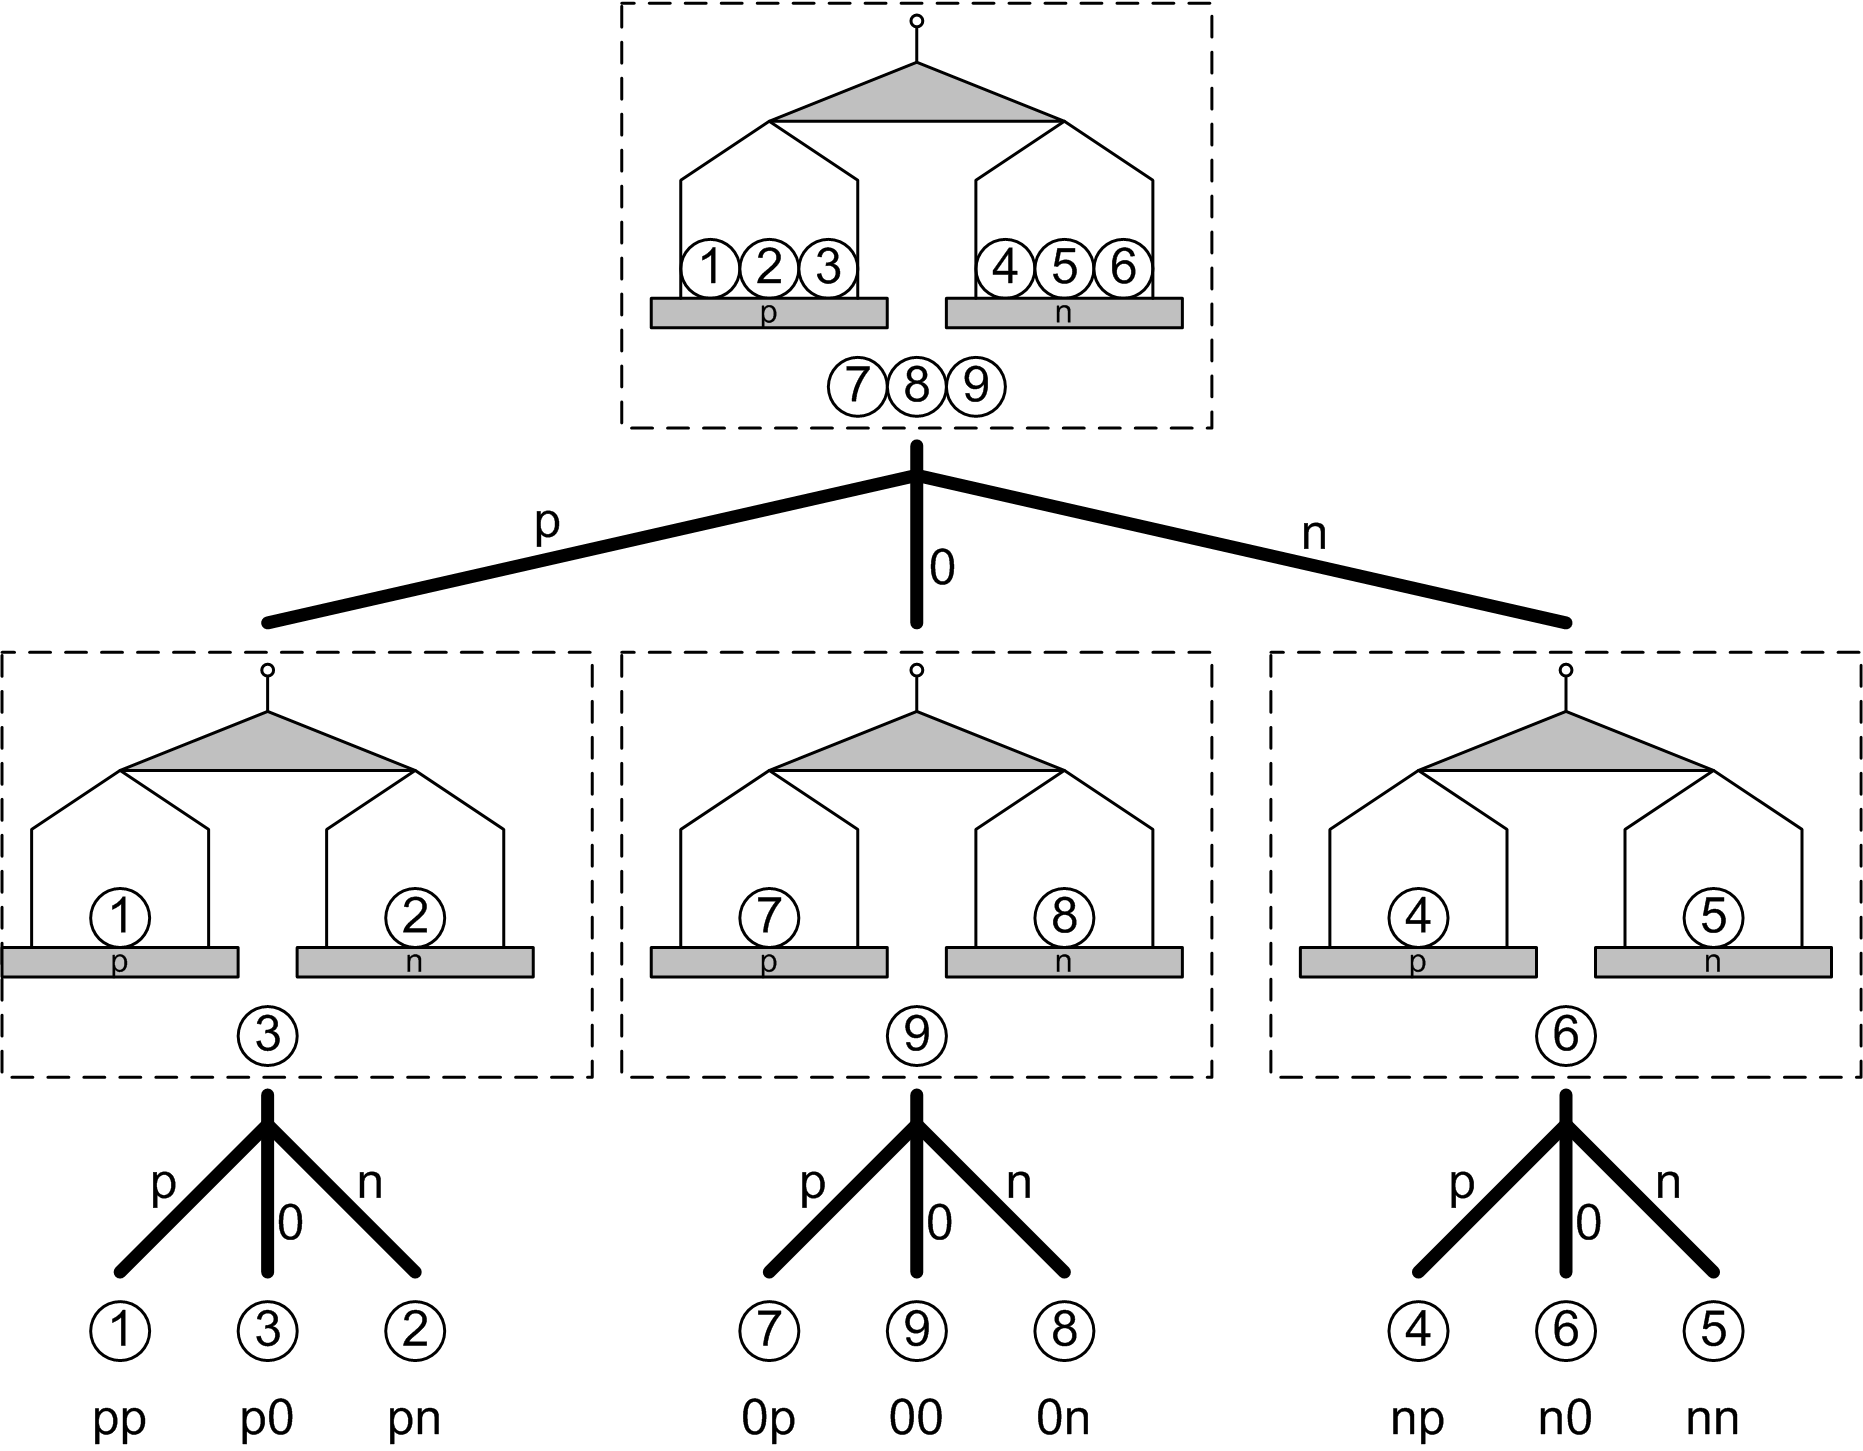
\includegraphics[height=.7\textheight]{pict/trit} }
        \mode<article>{ 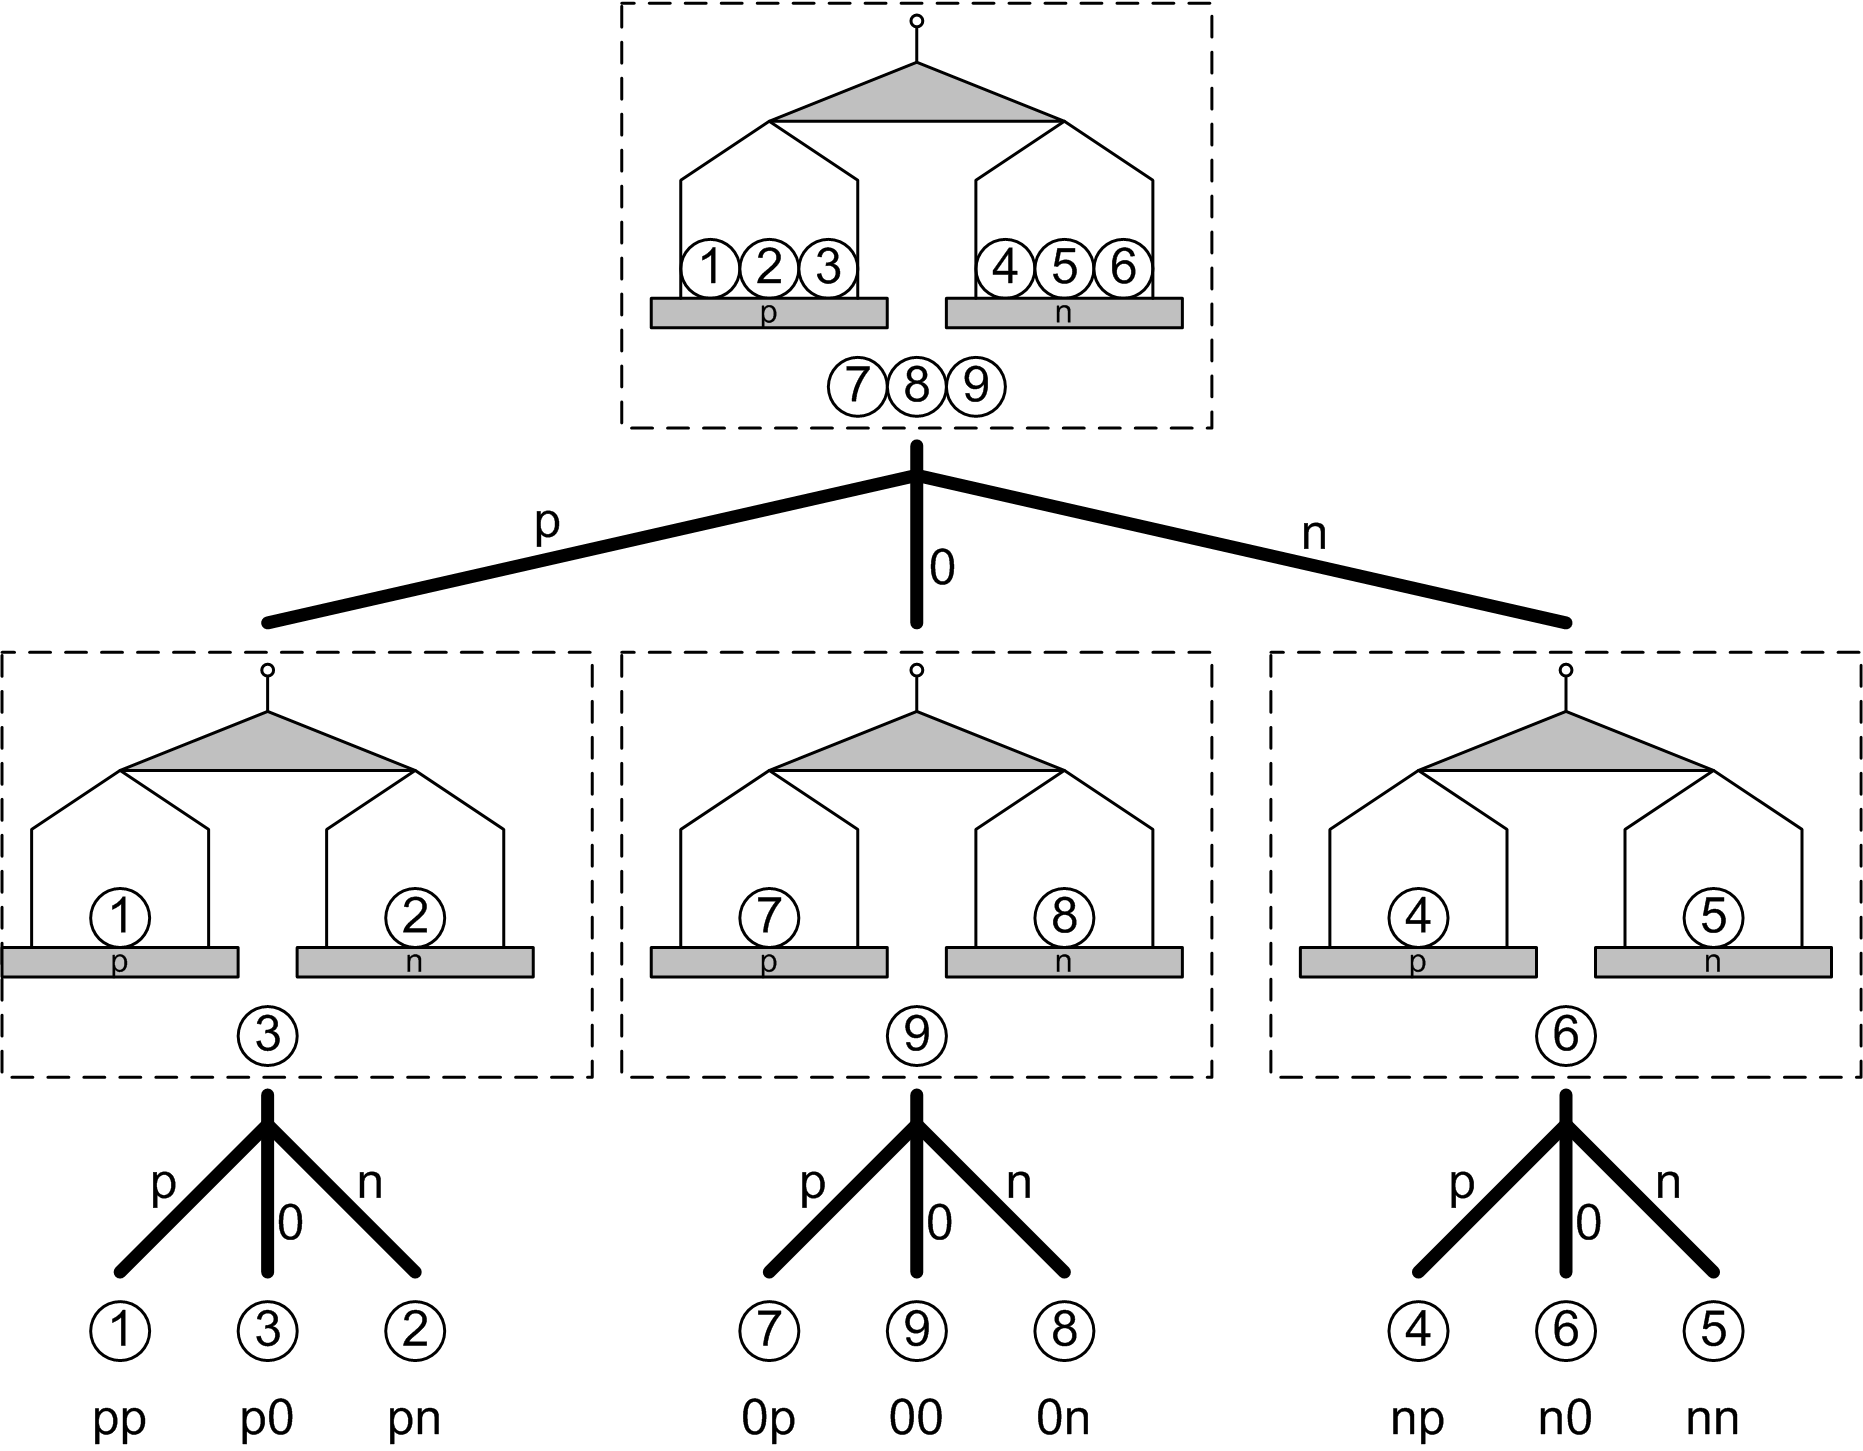
\includegraphics[width=.7\textwidth]{pict/trit} } 
    \end{center}
    \caption{Задача о биллиардных шарах}\label{pict:trit}
\end{figure} 
\mode<article>{ См. рисунок \ref{pict:trit} }
\end{frame}


\subsection{Семантический подход}

Отражаемый объект рассматривается как источник сообщений, которые для потребителя этих сообщений несут определенную смысловую нагрузку. Поэтому оценка адекватности информации зависит в первую очередь от способности потребителя принимать (понимать, воспринимать) сообщения\footnote{Звонок в службу поддержки оператора сотовой связи. Клиент: <<Девушка, до меня не доходят sms сообщения!!!>>.  Девушка: <<Прочтите еще раз\ldots>>. Бородатый анекдот.}. 

Обсуждая синтаксический подход, мы приводили пример двух сообщений, несущих разное (с точки зрения синтаксического подхода) количество информации: <<Жучка укусила Иванова>> и <<Иванов укусил Жучку>> и просили сравнить ощущения. Теперь сравните свои ощущения от следующих двух сообщений: <<бутявка укусила калушу>> и <<калуша укусила бутявку>>\footnote{Цикл лингвистических сказок <<Пуськи бятые>> Петрушевской Людмилы Стефановны}. Не доходят сообщения? Ноль адекватной информации в обоих случаях? Вероятно, это происходит потому, что в вашем личном тезаурусе нет определения смысла для <<бутявки>> и <<калуши>>, а также неизвестно в каких отношениях они находятся.

Слову <<тезаурус>> есть много определений. От древнегреческого: <<словарь с примерами>>, до современного лаконичного: <<совокупность выражающих смысл единиц языка с описанием отношений между ними>>. Оценки на основе тезауруса получили наибольшее распространение. При этом в большинстве случаев предполагается, что получатель получает именно информацию (цепочку символов), а не наблюдает события (то есть отражение уже свершилось). Следовательно, под сообщением понимается информация, а не событие.

Тезаурус пользователя мы обозначим $S_p$. Если $S_p$ пуст ($S_p=\emptyset$), то пользователь не понимает (не воспринимает) информацию и для него она --- информационный шум. Ежели $S_p$ всеобъемлющ ($S_p\rightarrow\infty$), то пользователь знает все, и ему нет необходимости понимать (воспринимать) информацию, так как она уже не обогатит его тезаурус. 

В большинстве случаев тезаурус пользователя находится между этими крайностями ($\emptyset<S_p<\infty$) и в этом случае поступающую информацию можно разделить на три части. Допустим, что потребитель получает информационную цепочку определенной длины ($I$). Причем в этой цепочке можно выделить фрагменты, несущие смысловые единицы и отношения которые: уже имеются в тезаурусе пользователя ($I_s$); отсутствуют в тезаурусе, но поняты (восприняты) и обогатят тезаурус ($I_c$); не поняты и представляют собой бесполезный информационный шум ($I_n$). Если длина фрагмента $I_n=0$, то поступающая информация идеально согласована с тезаурусом пользователя. При этом важной основной оценкой является коэффициент содержательности
\[C=\frac{I_c}{I}.\]
Как видно, этот коэффициент представляет собой отношение количества новой, осмысленной информации к общему её количеству.

\begin{frame}
\frametitle{Семантический подход}
\[I=I_s + I_c + I_n.\]
где $I_s$ --- известна, $I_c$ --- неизвестна и понятна, $I_n$ --- шум. $C=\frac{I_c}{I}$ называется коэффициентом содержательности информации.
\begin{figure}
    \begin{center}
        \mode<presentation>{ 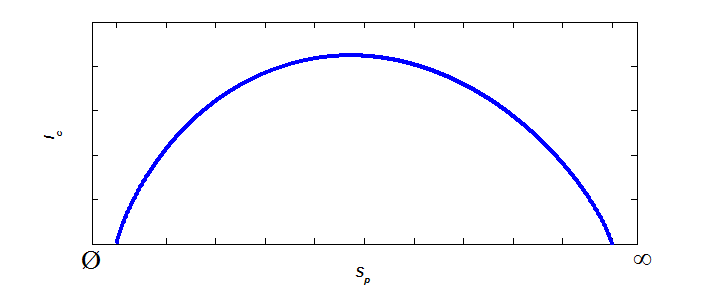
\includegraphics[height=.45\textheight]{pict/semantic} }
        \mode<article>{ 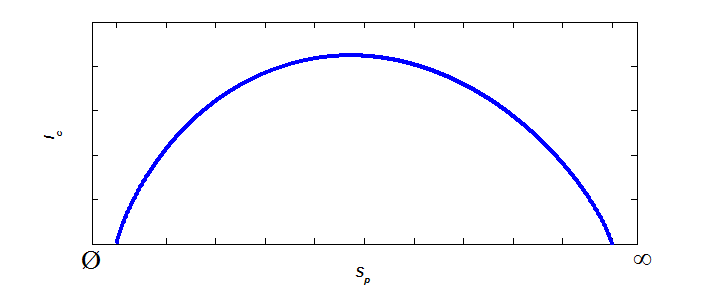
\includegraphics[width=.7\textwidth]{pict/semantic} } 
    \end{center}
    \caption{Зависимость $I_c$ в сообщении от тезауруса $S_p$ получателя}\label{pict:semantic}
\end{figure} 
\mode<article>{ См. рисунок \ref{pict:semantic} }
\end{frame}

Семантический подход учитывает особенности конкретного потребителя и дает количественную оценку адекватности информации с точки зрения её «осмысленности» для него. Одно и то же сообщение может оказаться полезным для компетентного, бессмысленным для некомпетентного и ненужным для всезнающего получателя. Внимание уделяется такой категории, как знание, а информация в данном случае --- это всего лишь способ (транстпорт) доставки знаний до познающего потребителя.


\subsection{Прагматический подход}

Как уже было сказано, прагматический подход количественно оценивает адекватность информации в контексте достижения потребителем какой-либо цели. Иными словами, дается количественная оценка ценности (целесообразности) информации для потребителя. В качестве примера приведем оценку советского ученого Александра Александровича Харкевича (1904-1965):

\begin{frame}
\frametitle{Прагматический подход}
\framesubtitle{Оценка Александра Александровича Харкевича}
\begin{equation}
    I=\log_{m}\frac{p_2}{p_1}=\log_{m}p_2 - \log_{m}p_1,
\end{equation}
где $m$ --- основание логарифма, определяющее единицы измерения ($m>1$), $p_1$ --- вероятность достижения потребителем \alert{цели} до получения информации, $p_2$ --- вероятность достижения потребителем цели после получения информации. Ценность информации в случае $p_1>p_2>0$ положительна, в случае $0<p_1<p_2$ отрицательна, а в случае $p_1=p_2$ равна нулю.
\end{frame}

В заключение следует отметить, что результаты оценок синтаксического подхода являются наиболее объективными, так как учитывают только отражаемый объект и избавлены от влияний со стороны конкретного потребителя, что характерно для остальных подходов.


\section{Кодирование}


Прежде чем продолжить разговор, четче разделим некоторые понятия, которые плотным кольцом окружают обсуждаемую тему кодирования. Под кодированием мы будем понимать процесс перехода от отражаемого объекта к набору символов (информации). При этом отражаемый объект – это источник значимых для нас событий. Ничто не мешает рассматривать набор символов (информацию) как отражаемый объект, когда требуется закодировать исходный набор символов по-другому (например, уменьшить его размер, сжать).


\begin{frame}
\frametitle{Кодирование}
\begin{definition}
    Под \alert{кодированием} мы будем понимать процесс перехода от \alert{отражаемого объекта} к совокупности (цепочке) \alert{символов} (т.е. к информации)
\end{definition}
Некоторые назначения кодирования:
\begin{enumerate}
    \item принципиальная возможность описания мира с помощью символов конечного алфавита;
    \item устранение избыточности, сжатие информации, экономия памяти и снижение нагрузки на каналы передачи информации;
    \item обеспечение помехоустойчивости;
    \item защита важных свойств информации.
\end{enumerate}
\end{frame}


\subsection{Сигналы}

Другим важным понятием является сигнал. Сигнал – это изменение (во времени или пространстве) физической величины, несущее информацию, т.е. способ, позволяющий фиксировать символ в материально-энергетическом носителе. Различают аналоговые (непрерывные) и цифровые (дискретные) сигналы. Соответственно различают аналоговую и цифровую технику. В чем принципиальная разница между аналоговым и цифровым сигналом?

\begin{frame}
\frametitle{Сигнал}
\begin{definition}
    \alert{Сигнал} --- это изменение (во времени или пространстве) физической величины, несущее информацию, т.е. способ, позволяющий фиксировать \alert{символ} в материально-энергетическом носителе
\end{definition}
Выделяют два вида сигналов:
\begin{enumerate}
    \item аналоговые;
    \item цифровые.
\end{enumerate}
\end{frame}


Представьте, что нужно передать, например, звук. Звук это сигнал – изменение физической величины «давления воздуха» в определенной точке (пусть в ухе) во времени. Это непрерывное изменение: для любого момента на оси времени можно определить значение давления. Увы, этот сигнал для передачи на большие расстояния не годится, требуется информацию передаваемую звуком представить другим сигналом, более удобным для передачи на большие расстояния.

Итак, путь первый, аналоговый. Заместить исходный сигнал более подходящим аналогом. Например, раскрутить со скоростью 33 оборота в секунду виниловый диск и алмазной иглой, которая благодаря мембране, повторяющей колебания воздуха, прочертит на виниле спиральную дорожку – пространственный аналог звука. Дальше такой сигнал можно передавать самолетом или поездом. Конечно, способов создать аналог масса, например, можно модулировать радиоволну звуковыми колебаниями. См. Рис. \ref{pict:analog}  Конечно, корень аналог не подразумевает, что аналоговый сигнал обязательно является непрерывным, но исторически так сложилось.

\begin{frame}
\frametitle{Аналоговый сигнал}
\begin{figure}
    \begin{center}
        \mode<presentation>{ 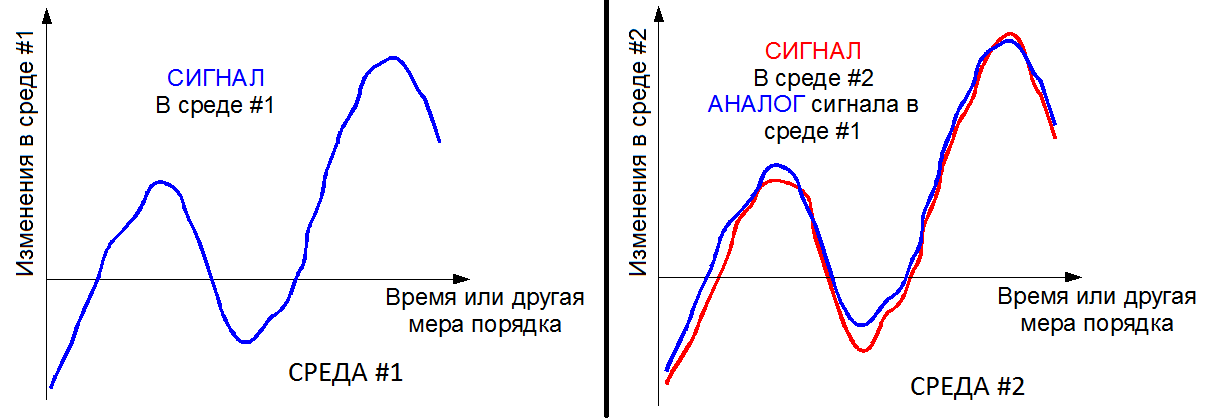
\includegraphics[width=\textwidth]{pict/analog} }
        \mode<article>{ 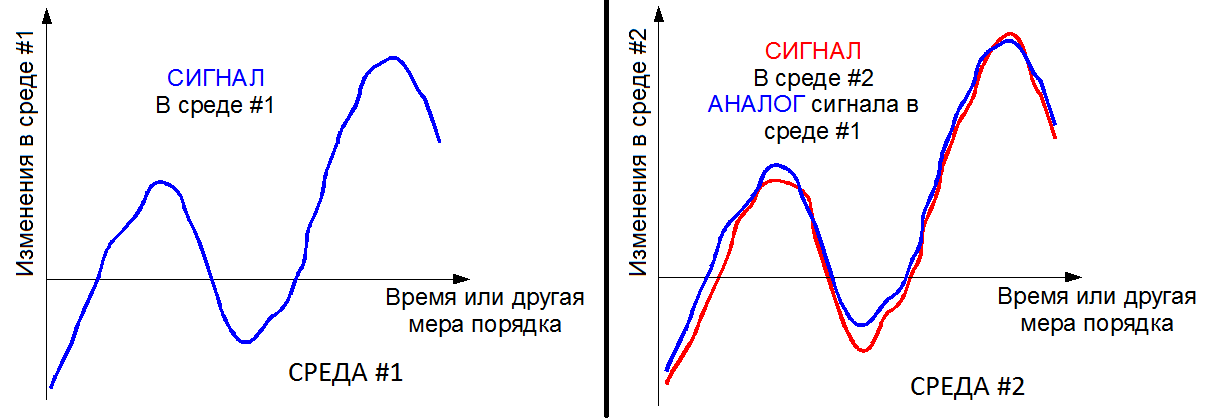
\includegraphics[width=.7\textwidth]{pict/analog} } 
    \end{center}
    \caption{Аналоговый сигнал}\label{pict:analog}
\end{figure} 
\mode<article>{ См. рисунок \ref{pict:analog} }
\end{frame}


Цифровой сигнал по определению прерывен, дискретен. Он содержит значения изменяющейся физической величины только в определенных точках времени или пространства. Значение физической величины определяется числом. Продолжая пример со звуком можно выполнить замеры давления воздуха в определенные моменты времени. Чем меньше промежуток между этими моментами, тем лучше. Получив набор чисел, их можно закодировать с помощью конечного набора символов-цифр. На Рис. \ref{pict:digital} числа закодированы в двоичной системе счисления (используются только два символа-цифры <<1>> и <<0>>).


\begin{frame}
\frametitle{Цифровой сигнал}
\begin{figure}
    \begin{center}
        \mode<presentation>{ 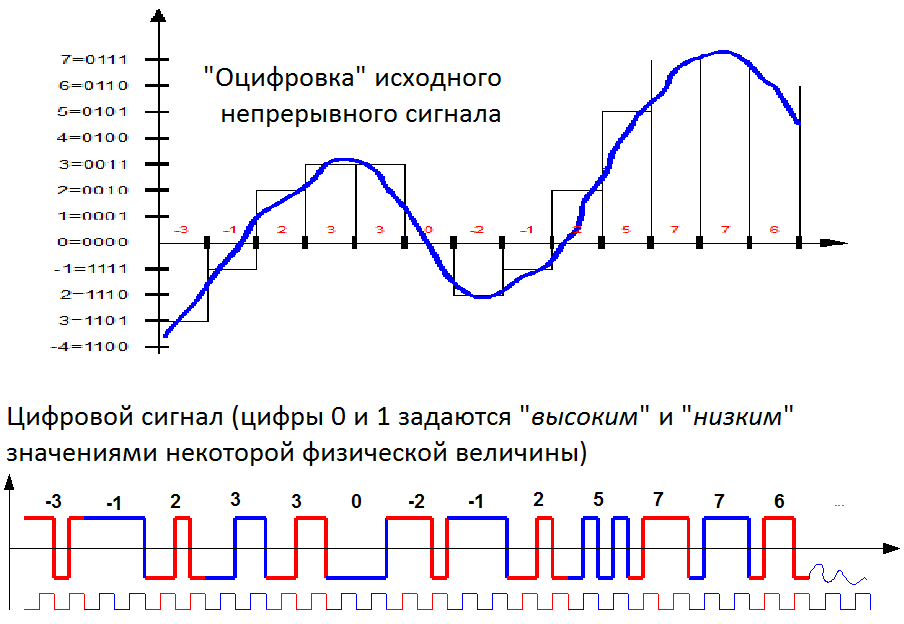
\includegraphics[height=.75\textheight]{pict/digital} }
        \mode<article>{ 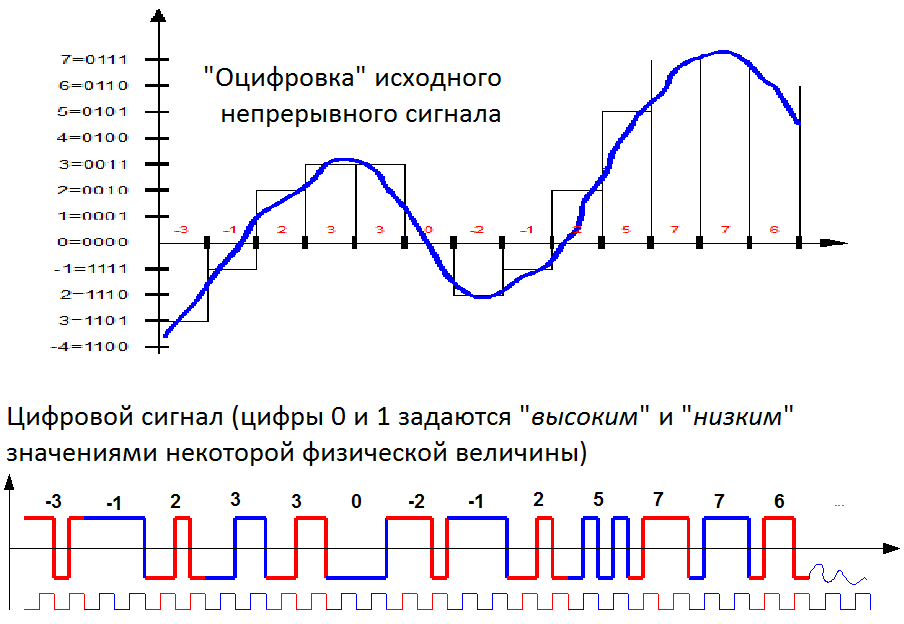
\includegraphics[width=.7\textwidth]{pict/digital} } 
    \end{center}
    \caption{Цифровой сигнал}\label{pict:digital}
\end{figure} 
\mode<article>{ См. рисунок \ref{pict:digital} }
\end{frame}


Естественно, цифровая форма представления по определению менее качественна, но обладает одним замечательным достоинством: число можно закодировать на носителе с $m$ устойчивыми состояниями (2-мя в современной технике), которые практически невозможно спутать. Поэтому цифровой сигнал намного более устойчив к помехам. Тысячная копия с копии лазерного диска (цифровой сигнал) будет идентичной оригиналу, а уже на сотой производной копии грампластинки вы не услышите ничего, кроме шума. Еще одно преимущество цифрового кодирования информации --- возможность использования всей мощи математики, для представления и обработки информации. Вычислительный узел, изначально предназначенный лишь для проведения сложных математических расчетов, в наше время играет ведущую роль в любых манипуляциях с цифровым представлением информации (например, очистка от помех, сжатие и т.д.)

Цифровая техника в настоящее время сильно потеснила аналоговую, но ценители качества, например меломаны, тяготеют к изделиям, в названии которых еще остается вхождения заветного корня <<аналог>>.

И хоть в процессе перехода от одного сигнала к другому иногда требуется кодирование (сигнал рассматривается как отражаемый объект) определения цифровое и аналоговое к кодированию отношения не имеют.


\subsection{Формальное определение кодирования}


\begin{frame}
\frametitle{Формальное определение кодирования}
\begin{definition}
    Дано:
    \begin{itemize}
        \item Алфавит \alert{событий}: $S=\{s_1,\ldots,s_N\}$;
        \item Алфавит кодовых \alert{символов}: $A=\{a_1,\ldots,a_m\}$;
    \end{itemize}
    
    Требуется задать соответствие:
    \[\delta=\langle s_1\to \omega_1,\ldots,s_N\to \omega_N\rangle,\]
    где $\omega_i=a_{i_1}\cdots a_{i_k}$, причем слово $\varsigma_j=s_{j_1}\cdots s_{j_t}$ будет кодироваться символами кодового алфавита как $\varsigma_j=\omega_{j_1}\cdots \omega_{j_t}$.
    Множество кодовых слов $\omega_i$, соответствующих $s_i$ называется множеством \alert{элементарных} кодов:
    \[\Omega=\{\omega_1,\ldots,\omega_N\}\]
\end{definition} 
\end{frame}


В общем случае имеется множество (алфавит) событий:
\[S=\{s_1,\ldots,s_N\},\]
где $s_i$ --- буква алфавита событий, которые требуется закодировать; $s_i$ обозначает отдельное событие; $N$ --- количество букв алфавита событий $S$.

Алфавит кодовых символов:
\[A=\{a_1,\ldots,a_m\},\]
где $a_i$ --- буква кодового алфавита (символ), а $m$ --- количество символов в алфавите символов $A$.

Требуется задать соответствие (схему, таблицу кодов) $\delta$ между событием $s_i$ и кодовым словом $\omega_i=a_{i_1}\cdots a_{i_k}$:
\[\delta=\langle s_1\to \omega_1,\ldots,s_N\to \omega_N\rangle,\]
причем слово $\varsigma_j$, состоящее из букв алфавита $S$ (т.е. набор событий):
\[\varsigma_j=s_{j_1}\cdots s_{j_t}\]
будет кодироваться символами кодового алфавита как
\[\varsigma_j=\omega_{j_1}\cdots \omega_{j_t}.\]
Множество кодовых слов $\omega_i$, соответствующих $s_i$ называется множеством элементарных кодов.
\[\Omega=\{\omega_1,\ldots,\omega_N\}\]


\begin{frame}
    \frametitle{Примеры кодирования}

    \begin{example}[Неоднозначное декодирование]
        $S=\{A,B,C,D,E,F,G,H\}$; $A=\{0,1\}$; $\delta=\langle A\to 0,B\to 1,C\to 10,D\to 11,E\to 100,F\to 101,G\to 110,H\to 111 \rangle$. \\Слову $ABAB$ однозначно соответствует цепочка $0101$. Но вот цепочке $0101$ помимо исходного $ABBA$, соответствуют слова $AF$ и $ACB$.
    \end{example} 

    \begin{example}[Однозначное декодирование]
        $S=\{A,B,C,D,E,F,G,H\}$; $A=\{0,1\}$; $\delta=\langle A\to 000,B\to 001,C\to 010,D\to 011,E\to 100,F\to 101,G\to 110,H\to 111 \rangle$. \\Слову $ABBA$ однозначно соответствует цепочка $000111000111$. И цепочке $000111000111$ также соответствует только  исходное $ABBA$.
    \end{example} 
\end{frame}


\begin{frame}
\frametitle{Схемы кодирования}

\begin{definition}
    Схема кодирования $\delta$ является \alert{разделимой}, если любое слово $\varsigma$, составленное из элементарных кодов $\omega_i$ единственным образом разлагается на элементарные коды.
\end{definition} 
Разделимая схема допускает декодирование. Важным частным случаем \alert{разделимых} схем являются \alert{префиксные} схемы.
\begin{definition}
    Схема называется \alert{префиксной}, если ни один элементарный код $\omega_i$ из множества $\Omega$ не является префиксом другого кода из того же множества.
\end{definition} 
\end{frame}

Префиксом, началом или приставкой слова $\omega$ называется слово $\omega_1$, если $\omega=\omega_1\omega_2$. Постфиксом или окончанием называется, соответственно, слово $\omega_2$. Коды, полученные на основе кодирующего дерева, пример кодированя в задаче о картах.


\subsection{Оптимальное кодирование}


\begin{frame}
\frametitle{Энтропия}
Энтропия источника \alert{событий} $s_i\in S$ с вероятностью появления $p_i$:
\[E=-\sum_{i=1}^{N}p_{i}\cdot \log_{m}p_i.\]
Энтропия соответствующего ему источника \alert{информации}:
\[E=\sum_{i=1}^{N}p_{i}\cdot I_i,\]
где $I_i$ --- количество информации, соответствующее $s_i$ (т.е. длина кодового слова $\omega_i$). Энтропия эквивалентного источника информации всегда больше энтропии источника сообщений.
\end{frame}


\begin{frame}
\frametitle{Энтропия}
\begin{example}
    \begin{table}[ht]
    \caption{Варианты кодирования стационарного источника}
    \label{t:optStatSource}
    \centering
    \begin{tabular}[c]{|l|l|l|l|l|}
        \hline
        Событие $s_i$                       &А      &Б      &В      &Г    \\ \hline
        Вероятность $p_i$ события $s_i$     &0.5    &0.3    &0.1    &0.1  \\ \hline
        \hline
        1-й код события $\omega_i$          &00     &01     &10     &11   \\ \hline
        2-й код события $\omega_i$          &0      &10     &110    &111  \\ \hline
    \end{tabular}
    \end{table}
\mode<article>{Cтационарный источник представлен в таблице \ref{t:optStatSource}}
\end{example}
$E_S=-(0.5\cdot \log_2 0.5+0.3\cdot \log_2 0.3+0.1\cdot \log_2 0.1+0.1\cdot \log_2 0.1)\approx 1.69$.\\
$E_{I_1}=-(0.5\cdot 2+0.3\cdot 2+0.1\cdot 2+0.1\cdot 2)=2$.\\
$E_{I_2}=-(0.5\cdot 1+0.3\cdot 2+0.1\cdot 3+0.1\cdot 3)=1.7$.\\
В случае передачи 100 символов, экономия $I_2$ по сравнению с $I_1$ составит примерно 30 бит.
\end{frame}

Результаты 2-го источника много лучше! Так, если запустить источники информации на выдачу, например, 100 символов то первый вариант кодирования выдаст нам цепочку длины примерно $50\cdot 2+30\cdot 2+10\cdot 2+10\cdot 2=200$ бит. А второй примерно $50\cdot 1+30\cdot 2+10\cdot 3+10\cdot 3=170$ бит. Экономия при том же качестве, как говорится, налицо! Лучший ли это результат? Как же закодировать источник действительно оптимальным образом? Рассмотрим алгоритма оптимального кодирования Хаффмана.


\begin{frame}
\frametitle{Алгоритм Хаффмана для $m=2$}
\begin{enumerate}
    \item\label{enumer:haffSort} События сортируются по убыванию вероятности.
    
    \item\label{enumer:haffGlue} Два события с минимальными вероятностями объединяются в одно составное событие, которое имеет вероятность, равную сумме вероятностей исходных. При этом одно из исходных событий помечается кодовым символом 0, а второе --- символом 1. Исходные события исключаются из множества событий, вместо них остается одно составное. 
    
    \item Шаги \ref{enumer:haffSort} и \ref{enumer:haffGlue} последовательно повторяются до тех пор, пока все события не склеятся в единственное составное событие (корень), вероятность которого, очевидно, равна 1. После этого кодовое слово $\omega_i$ для исходного события $s_i$ есть цепочка из кодовых символов, которыми помечены все составные события от корня до $s_i$ 

\end{enumerate}
\end{frame}


\begin{frame}
\frametitle{Алгоритм Хаффмана}
\framesubtitle{Закодируйте стационарный источник}
\begin{example}
    \begin{table}[ht]
    \caption{Стационарный источник}
    \label{t:haffStatSource}
    \centering
    \begin{tabular}[c]{|l|l|l|l|l|l|}
        \hline
        Событие $s_i$                       &А      &Б      &В      &Г     &Д     \\ \hline
        Вероятность $p_i$ события $s_i$     &0.5    &0.125  &0.125  &0.125 &0.125 \\ \hline
    \end{tabular}
    \end{table}
    \mode<article>{Cтационарный источник представлен в таблице \ref{t:haffStatSource}}
\end{example}
\end{frame}


\begin{frame}
\frametitle{Алгоритм Хаффмана}
\framesubtitle{Кодирование источника}
\begin{figure}
    \begin{center}
        \mode<presentation>{ 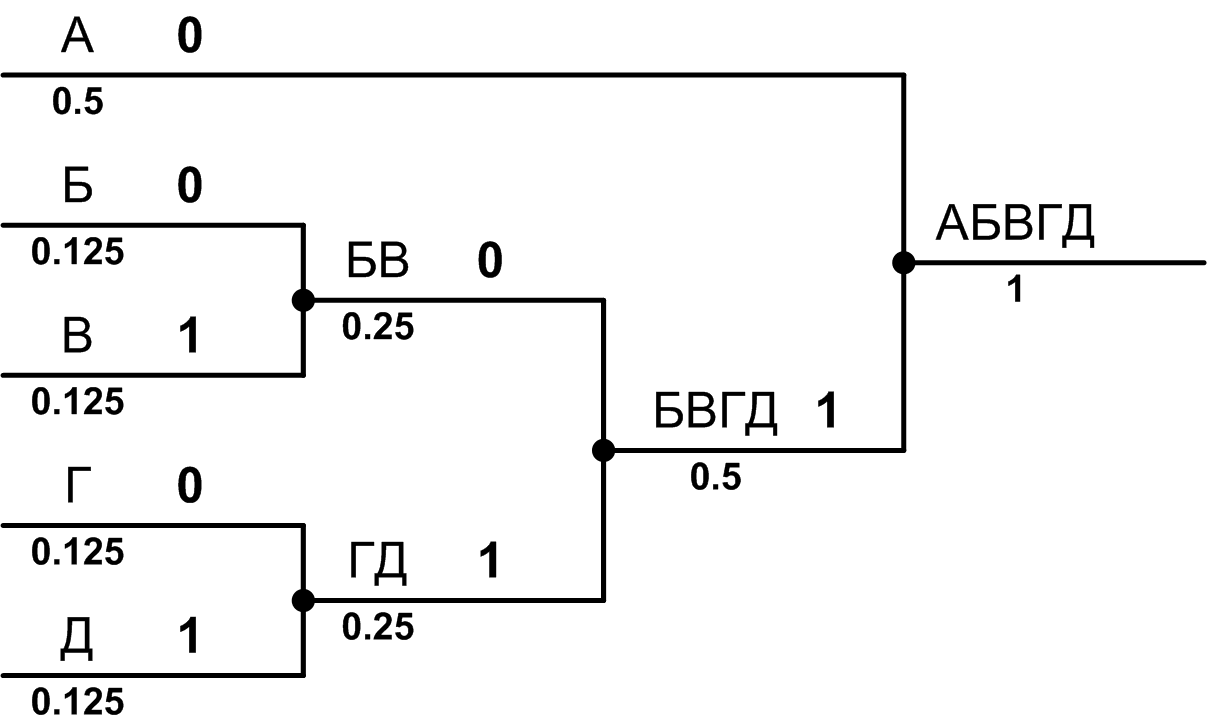
\includegraphics[height=0.7\textheight]{pict/huffman} }
        \mode<article>{ 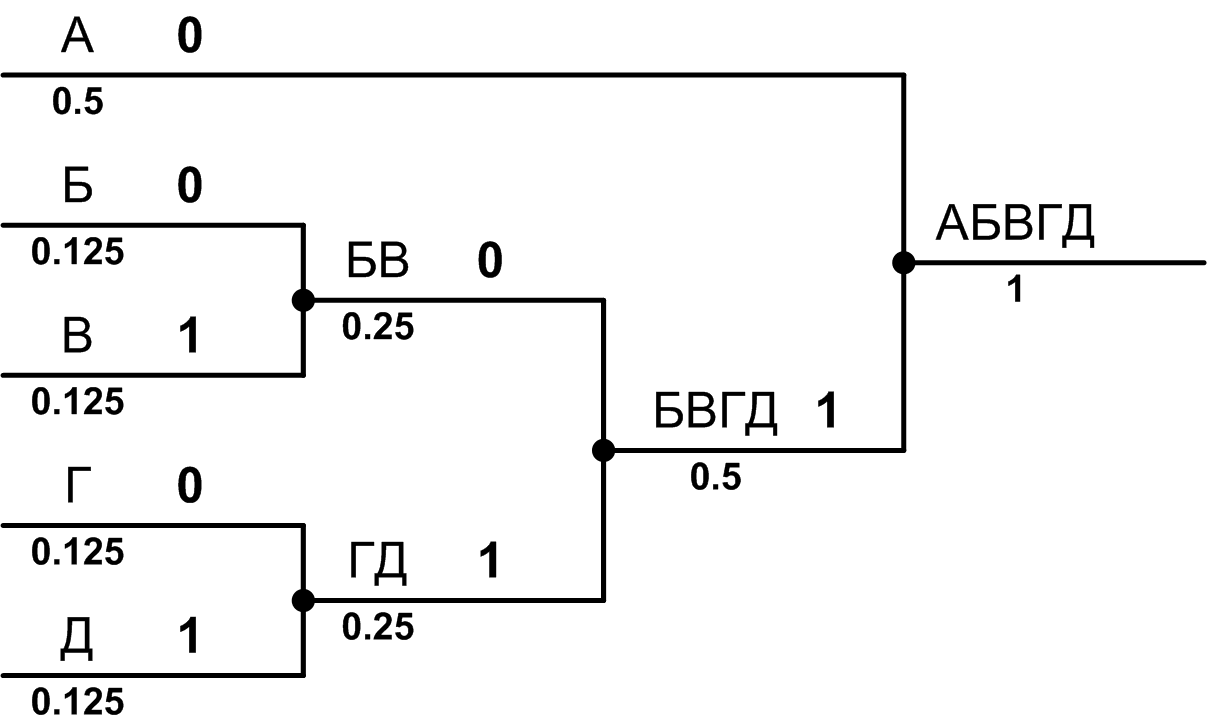
\includegraphics[width=.7\textwidth]{pict/huffman} } 
    \end{center}
    \caption{Алгоритм Хаффмана: кодирование}\label{pict:huffman}
\end{figure} 
\mode<article>{ См. рисунок \ref{pict:huffman} }
\end{frame}


\begin{frame}
\frametitle{Алгоритм Хаффмана}
\framesubtitle{Результат кодирования}
\begin{example}
    \begin{table}[ht]
    \caption{Результат кодирования источника}
    \label{t:haffStatSourceResult}
    \centering
    \begin{tabular}[c]{|l|l|l|l|l|l|}
        \hline
        Событие $s_i$                       &А      &Б      &В      &Г      &Д     \\ \hline
        Вероятность $p_i$ события $s_i$     &0.5    &0.125  &0.125  &0.125  &0.125 \\ \hline\hline
        Код события $\omega_i$              &0      &100    &101    &110    &111   \\ \hline
    \end{tabular}
    \end{table}
    \mode<article>{Cтационарный источник представлен в таблице \ref{t:haffStatSourceResult}}
\end{example}
Получен префиксный код? Попробуйте декодировать информацию: 10001101110111. Оцените энтропию источника событий и соответствующего источника информации.
\end{frame}


\section{Сжатие данных}


\begin{frame}
\frametitle{Классы алгоритмов сжатия данных}
\begin{definition}
    \alert{Информация}, для которой известно как её интерпретировать, называется \alert{данными}. \alert{Сжатие} данных --- уменьшение количества несущей информации, с сохранением (порой частичным) свойства \alert{адекватности} отражаемому объекту.
\end{definition}
\begin{itemize}
    \item С потерями (JPEG, MPEG (MP3, MP4), \ldots).
    \item Без потерь (RLE, LZx, арифметическое,\ldots).
    \begin{itemize}
        \item Статистические.
        \item Словарные.
        \item\ldots
    \end{itemize}
\end{itemize}
Для сжатия разных видов \alert{данных} (например, текста, изображений, видео, звука и т.д.) применяются весьма специфичные алгоритмы сжатия. 
\end{frame}


\subsection{Алгоритм Лемпела-Зива}


Мы уже рассматривали способы оптимального кодирования информации. Но не всегда информация отражает объект оптимальным образом (иногда в этом нет необходимости) и количество информации превышает необходимый минимум. В этом случае говорят об избыточности информации. Но очень часто требуется уменьшить количество информации, сжать её в целях экономии ресурсов памяти или снижения нагрузки на каналы передачи. Методы оптимального кодирования активно используются при сжатии информации, так, например, многие алгоритмы сжатия изображений используют алгоритм Хаффмана.

Итак, чётче разделим понятия оптимальное кодирование и кодирование с целью сжатия. Оптимальное кодирование ставит себе в задачу сопоставить отражаемому объекту минимальное количество адекватной ему информации. Кодирование с целью сжатия ставит себе в задачу уменьшить количество информации, не теряя (или оставаясь в допустимых рамках) при этом свойство адекватности. Кодирование с целью сжатия будем далее называть просто сжатие. В случае сжатия, отражаемым объектом выступает информация, причем события $s_i$ в этом случае представляют собой слова в алфавите $A$. То есть информация перекодируется в том же алфавите $A$.

Выделяют два больших класса алгоритмов сжатия информации: сжатие с потерями и без потерь. <<Теряется>>, конечно, адекватность. При сжатии без потерь из сжатой информации можно восстановить исходную информацию в точности такую же, как до сжатия. При сжатии с потерями восстановленная информация будет отличаться от исходной. Ярким примером сжатия с потерями является сжатие изображений: используя определенные особенности восприятия цвета человеком, такие алгоритмы отбрасывают <<лишнюю>> информацию. Потеря адекватности отражаемому объекту в этом случае значительная, но для человека-потребителя эти потери адекватности незаметны.

Часто алгоритмы сжатия весьма специфичны и учитывают особенности отражаемого объекта (как в случае изображений). Важнейшим отражаемым объектом в жизни человека является речь, текст. На основе, например, русского алфавита можно построить бесконечное количество слов, но в реальной жизни словарный запас редко превышает сотню тысяч слов. На практике для универсального представления текста байтами кодируются буквы, цифры, знаки препинания, пробелы и т.д., но если мы знаем, что кодируется именно осмысленный текст (содержащий осмысленные слова), то можно сильно сэкономить, кодируя в качестве сообщений $s_i$ не буквы, а слова. Такие методы сжатия называются словарными. 

Впрочем, словарные методы могут использоваться не только для кодирования текста, но для произвольных информационных цепочек. Причем словарь может строиться динамически и совершенно не учитывать смысловой нагрузки слов в словаре.

Рассмотрим один из методов словарного сжатия: алгоритм Лемпела-Зива. Существует множестово его модификаций: LZ77, LZSS, LZ78, LZW.

В основе алгоритма Лемпела-Зива лежит идея адаптивного сжатия. За один проход по тексту одновременно строится и словарь и код, причем словарь не хранится, так как при декодировании он динамически восстанавливается. Мы рассмотрим кодирование и декодирование на примере, при этом допустим, что для кодирования букв (цифр, знаков препинания и т.д.) текста используется байт. Для хранения индекса слова в словаре также будет использоваться байт.


\begin{frame}
\frametitle{Алгоритм Лемпела-Зива}
\framesubtitle{Кодирование (сжатие). Модификации, используемые на практике: LZ77, LZSS, LZ78, LZW}
\begin{enumerate}
    \item В словарь нулевым элементом помещается пустое слово $\varepsilon$. Пустое слово $\varepsilon$ не содержит букв и для любого слова $s$ справедливо $s=\varepsilon s=s\varepsilon$.
    \item \label{enumer:LZWsasplit} От исходного текста $t$ отделяется слово $sa$, где $s$ --- максимально длинное слово из словаря; $a$ --- расширяющая буква. Т.е. $t=sat'$.
    \item \label{enumer:LZWsaadd} В словарь добавляется новое слово $sa$. К коду $c$ добавляется пара $\langle i_s,a\rangle$, где $i_s$ --- индекс слова $s$ в словаре. От исходного текста отделяется слово $sa$: $t\gets t'$.
    \item Пункты \ref{enumer:LZWsasplit}-\ref{enumer:LZWsaadd} последовательно повторяются до тех пор, пока в тексте $t$ остается хоть одна буква.
\end{enumerate}
\end{frame}


В результате получается код $c$, представляющий собой упорядоченное множество  пар $\langle\text{индекс,буква}\rangle$: $c=\{\langle i_1,a_1\rangle,\langle i_2,a_2\rangle,\ldots\}$.


\begin{frame}
\frametitle{Алгоритм Лемпела-Зива}
\framesubtitle{Декодирование}
\begin{enumerate}
    \item В словарь нулевым элементом помещается пустое слово $\varepsilon$. Текст $t$ не содержит букв: $t=\varepsilon$.
    \item \label{enumer:LZWsasplitadd} От исходного кода $c$ отделяется пара $\langle i,a\rangle$, в словарь добавляется слово $s_{i}a$, где $s_i$ --- $i$-е слово из словаря (словарь восстанавливается так же, как и формируется!). В конец текста добавляется слово $s_{i}a$:  $t\gets ts_{i}a$.
    \item Пункт \ref{enumer:LZWsasplitadd} последовательно повторяется до тех пор, пока в коде $c$ остается хоть одна пара.
\end{enumerate}
\end{frame}


Прежде, чем рассмотреть пример, нужно отметить, что данный алгоритм хорошо сжимает тексты большого объема, в которых так или иначе будут присутствовать одинаковые и достаточно длинные слова. В примере такие вхождения созданы искусственно. Для текстов малого объема, скорее всего, длина кода сжатого текста будет превышать длину кода для исходного текста.

\begin{frame}
\frametitle{Алгоритм Лемпела-Зива}
\framesubtitle{Пример сжания текста <<АБАКАНКАНКАНКИАНКИН>>}
\begin{table}[ht]
\caption{Сжатие:<<АБАКАНКАНКАНКИАНКИН>>}
\label{t:LZWEncode}
\centering
\begin{tabular}[c]{|l|l|l|l|}
\hline\hline
$i$ & $t$                                            & $sa$                         & $c=\langle i_s,a\rangle$ \\ 
\hline\hline
  &                                                  & $0\rightarrow\varepsilon $   & \\ \hline
1 &	$\varepsilon\text{\textbf{А}БАКАНКАНКАНКИАНКИН}$ & $1\rightarrow\text{A}    $   & $\langle\text{0,А}\rangle$ \\ \hline
2 &	$\varepsilon\text{\textbf{Б}АКАНКАНКАНКИАНКИН} $ & $2\rightarrow\text{Б}    $   & $\langle\text{0,Б}\rangle$ \\ \hline
3 &	$           \text{\textbf{АК}АНКАНКАНКИАНКИН}  $ & $3\rightarrow\text{АК}   $   & $\langle\text{1,К}\rangle$ \\ \hline
4 &	$           \text{\textbf{АН}КАНКАНКИАНКИН}    $ & $4\rightarrow\text{АН}   $   & $\langle\text{1,Н}\rangle$ \\ \hline
5 &	$\varepsilon\text{\textbf{К}АНКАНКИАНКИН}      $ & $5\rightarrow\text{К}    $   & $\langle\text{0,К}\rangle$ \\ \hline
6 &	$           \text{\textbf{АНК}АНКИАНКИН}       $ & $6\rightarrow\text{АНК}  $   & $\langle\text{4,К}\rangle$ \\ \hline
7 &	$           \text{\textbf{АНКИ}АНКИН}          $ & $7\rightarrow\text{АНКИ} $   & $\langle\text{6,И}\rangle$ \\ \hline
8 &	$           \text{\textbf{АНКИН}}              $ & $8\rightarrow\text{АНКИН}$   & $\langle\text{7,Н}\rangle$ \\ \hline
\end{tabular}
\end{table}
\mode<article>{Пример сжатия текста: «АБАКАНКАНКАНКИАНКИН» представлен в таблице \ref{t:LZWEncode}}
\end{frame}


Итак, полученный код (сжатый текст) занимает 8*2=16 байт информации (один байт на индекс, второй на букву), а код исходного текста занимает 19 байт (один байт на букву).

\begin{frame}
\frametitle{Алгоритм Лемпела-Зива}
    \framesubtitle{Пример декодирования <<0А0Б1К1Н0К4К6И7Н>>}
    
    \begin{table}[ht]
        \mode<article>{
            \caption{Декодирование:<<0А0Б1К1Н0К4К6И7Н>>}
            \label{t:LZWDecode}
        }
        \centering
        \begin{tabular}[c]{|l|l|l|l|}
            \hline\hline
            $i$ & $c=\langle i_s,a\rangle$ & $sa$                         & $t$ \\ 
            \hline\hline
              &                            & $0\rightarrow\varepsilon $   &                                                 \\ \hline
            1 & $\langle\text{0,А}\rangle$ & $1\rightarrow\text{A}    $   &	$\text{}      \varepsilon\text{\textbf{А}}    $ \\ \hline
            2 & $\langle\text{0,Б}\rangle$ & $2\rightarrow\text{Б}    $   &	$\text{А}     \varepsilon\text{\textbf{Б}}    $ \\ \hline
            3 & $\langle\text{1,К}\rangle$ & $3\rightarrow\text{АК}   $   &	$\text{АБ}               \text{\textbf{АК}}   $ \\ \hline
            4 & $\langle\text{1,Н}\rangle$ & $4\rightarrow\text{АН}   $   &	$\text{АБАК}             \text{\textbf{АН}}   $ \\ \hline
            5 & $\langle\text{0,К}\rangle$ & $5\rightarrow\text{К}    $   &	$\text{АБАКАН}\varepsilon\text{\textbf{К}}    $ \\ \hline
            6 & $\langle\text{4,К}\rangle$ & $6\rightarrow\text{АНК}  $   &	$\text{АБАКАНК}          \text{\textbf{АНК}}  $ \\ \hline
            7 & $\langle\text{6,И}\rangle$ & $7\rightarrow\text{АНКИ} $   &	$\text{АБАКАНКАНК}       \text{\textbf{АНКИ}} $ \\ \hline
            8 & $\langle\text{7,Н}\rangle$ & $8\rightarrow\text{АНКИН}$   &	$\text{АБАКАНКАНКАНКИ}   \text{\textbf{АНКИН}}$ \\ \hline
        \end{tabular}
    \end{table}
    \mode<article>{Декодирование (восстановление текста из кода) представлено в таблице \ref{t:LZWDecode}}
    \[
        \overbrace{\varepsilon}^0
        \overbrace{\text{А}}^1_{\langle 0,\text{А}\rangle}
        \overbrace{\text{Б}}^2_{\langle 0,\text{Б}\rangle}
        \overbrace{\text{АК}}^3_{\langle 1,\text{К}\rangle}
        \overbrace{\text{АН}}^4_{\langle 1,\text{Н}\rangle}
        \overbrace{\text{К}}^5_{\langle 0,\text{К}\rangle}
        \overbrace{\text{АНК}}^6_{\langle 4,\text{К}\rangle}
        \overbrace{\text{АНКИ}}^7_{\langle 6,\text{И}\rangle}
        \overbrace{\text{АНКИН}}^8_{\langle 7,\text{Н}\rangle}
    \]
\end{frame}

\begin{frame}
    \frametitle{Алгоритм Лемпела-Зива}
    \framesubtitle{Задание}
    
    Сжать текст:
    \[
        \text{<<тартарарамитамтамывтартарарах>>}
    \]
    \uncover<2>{
        \[
            \overbrace{\varepsilon}^0
            \overbrace{\text{т}}^1_{\langle 0,\text{т}\rangle}
            \overbrace{\text{а}}^2_{\langle 0,\text{а}\rangle}
            \overbrace{\text{р}}^3_{\langle 0,\text{р}\rangle}
            \overbrace{\text{та}}^4_{\langle 1,\text{а}\rangle}
            \overbrace{\text{ра}}^5_{\langle 3,\text{а}\rangle}
            \overbrace{\text{рам}}^6_{\langle 5,\text{м}\rangle}
            \overbrace{\text{и}}^7_{\langle 0,\text{и}\rangle}
            \overbrace{\text{там}}^8_{\langle 4,\text{м}\rangle}
            \overbrace{\text{тамы}}^9_{\langle 8,\text{ы}\rangle}
            \overbrace{\text{в}}^{10}_{\langle 0,\text{в}\rangle}
            \overbrace{\text{тар}}^{11}_{\langle 4,\text{р}\rangle}
            \overbrace{\text{тара}}^{12}_{\langle 11,\text{а}\rangle}
            \overbrace{\text{рах}}^{13}_{\langle 5,\text{х}\rangle}
        \]
        Код:
        \[
            \begin{split}
                \langle 0,\text{т}\rangle,
                \langle 0,\text{а}\rangle,
                \langle 0,\text{р}\rangle,
                \langle 1,\text{а}\rangle,
                \langle 3,\text{а}\rangle,
                \langle 5,\text{м}\rangle,
                \langle 0,\text{и}\rangle,\\
                \langle 4,\text{м}\rangle,
                \langle 8,\text{ы}\rangle,
                \langle 0,\text{в}\rangle,
                \langle 4,\text{р}\rangle,
                \langle 11,\text{а}\rangle,
                \langle 5,\text{х}\rangle
            \end{split}
        \]
    }
\end{frame}


\appendix


\section{Источники}
\begin{frame}
    \frametitle{Источники}

    Класификацию точек зрения на информацию, её свойств и подходов к оценке можно найти в любом учебнике по информатике, например, \cite{bib:ostreykovsky:informatics}.

    Основы кодирования, теория Клода Шеннона и её прикладное значение, включая алгоритмы оптимального кодирования: \cite{bib:panin:informationTheory, bib:verner:codingBase}.

    Ясное изложение алгоритма сжатия Лемпела-Зива можно найти в \cite{bib:novic:discrmathprogrammer} и подробно (включая модификации) в \cite{bib:salmon:compressing}.

    Сжатие различных видов данных кратко и ясно изложено в \cite{bib:salmon:compressing}.

    Рекомендован к прочтению закон №149-ФЗ от 27 июля 2006 г <<Об информации, информационных технологиях и о защите информации>>.

    О кодировании и вычислительной технике в популярном изложении: \cite{bib:petsold:code}

\end{frame}


\section{Вопросы для самопроверки}
\begin{frame}[allowframebreaks]{Вопросы для самопроверки}
    \begin{enumerate}
        \item Что такое информация?
        \item Какие существуют точки зрения на информацию? Дать краткое описание каждой точки зрения?
        \item Какие внутренние и внешние свойства вы знаете? В отношении каких объектов проявляются внешние свойства?
        \item Какие свойства информации наиболее важны с точки знения её защиты?
        \item Какие существуют подходы к количественной оценке информации?
        \item Сколько бит в байте?
        \item Какие единицы измерения информации вы знаете?
        \item Приведите пример сообщения имеющего нулевой коэффициент содержательности (семантический подход, нулевой и бесконечный тезаурус)?
        \item Приведите пример сообщения несущего информацию 1 бит и -1 бит (прагматический подход)?
        \item Что такое сигнал? Приведите отличия цифрового и аналогового сигналов.
        \item Чем оптимальное кодирование отличается от сжатия?
    \end{enumerate}
\end{frame}


\section{Библиоргафия}
%слайд раскладывается на несколько: allowframebreaks
\begin{frame}[allowframebreaks]{Библиография}
    \bibliographystyle{gost780u}
    \bibliography{./../bibliobase}
\end{frame}

\end{document}